\documentclass[11pt]{article}
\usepackage[margin=0.85in]{geometry}
\usepackage{booktabs,array,multirow}
\usepackage{amsmath,amssymb}
\usepackage{graphicx}
\usepackage[font=small,labelfont=bf]{caption}
\usepackage{enumitem}
\usepackage{xcolor}
\usepackage{hyperref}
\usepackage{subcaption}
\usepackage{float}
\usepackage{placeins}
\renewcommand{\topfraction}{0.95}
\renewcommand{\bottomfraction}{0.95}
\renewcommand{\textfraction}{0.05}
\renewcommand{\floatpagefraction}{0.7}
\setcounter{topnumber}{3}
\setcounter{bottomnumber}{3}
\setcounter{totalnumber}{6}

\setlength{\parskip}{0.35em}
\setlength{\parindent}{0em}
\hypersetup{colorlinks=true,linkcolor=blue!60!black,urlcolor=blue!60!black}

\title{\Large\textbf{GAD vs Sella on HIP --- Five-Method Comprehensive Benchmark}\\[4pt]
\normalsize 2026-04-20, Transition1x train, 300 samples $\times$ 6 noise levels, 2000 steps,
IRC validation via \texttt{sella\_hip}}
\author{}
\date{}

\begin{document}
\maketitle
\thispagestyle{empty}

\begin{center}
\fbox{\parbox{0.95\textwidth}{\small
\textbf{TL;DR.} Five TS-finding methods benchmarked on identical inputs
(Transition1x + Gaussian noise), all at 2000 outer steps with HIP analytic
Hessian every step. All evaluated under matched
$n_{\text{neg}}{=}1 \wedge f_{\max}{<}0.01$ criterion (canonical) plus an
independent \texttt{sella\_hip} IRC validation.

\textbf{At TS-finding (canonical fmax<0.01):} 200\,pm convergence rates:
GAD Eckart 45.3\%, GAD no-Eckart 43.3\%, Sella Cart variants 24--26\%,
Sella internal 17\%.

\textbf{At IRC validation (TOPO-intended, proportion of 300):} 200\,pm:
GAD Eckart 47.0\%, GAD no-Eckart 45.7\%, Sella Cart$\pm$Eckart 22--25\%,
Sella internal 19\%.

\textbf{Three findings (one is a correction).}
(1) Under the matched fmax criterion, \textbf{Sella Cartesian beats GAD by $\sim$4 pp at low noise}
(10--50\,pm), but GAD takes over decisively at 100\,pm and above
(crossover $\sim$80--100\,pm). The earlier ``GAD always wins'' picture was
inflated by GAD's looser force\_norm criterion.
(2) \textbf{Eckart projection contributes essentially nothing} for GAD
under fmax: same convergence rate ($\pm$1\,pp), same IRC outcomes
($>$95\% per-sample agreement), same step efficiency (within 5\%).
The ``Eckart is a step-efficiency multiplier'' claim from earlier
was an artifact of a mixed-criteria comparison; corrected here.
(3) Internal coordinates \emph{hurt} Sella on HIP by 12--30\,pp across
noise levels --- Sella's library default is the worst configuration tested.
}}
\end{center}

\tableofcontents
\newpage

% =================================================================
\section{Methodology}
% =================================================================

\subsection{Dataset and noise}

Transition1x train split, samples 0--299 (fixed 300-sample universe).
For each sample $i$ and noise $\sigma \in \{10,30,50,100,150,200\}$\,pm:
\[
\mathbf{x}_0^{(i,\sigma)} = \mathbf{x}_{\text{TS}}^{(i)} + \sigma \cdot \boldsymbol{\xi}_i,\;
\boldsymbol{\xi}_i \sim \mathcal{N}(0, I_{3N}),\;\text{seed}=42.
\]
HIP potential throughout (\texttt{hip\_v2.ckpt}); analytic Hessian; A100 MIG (2g.10gb).

\subsection{The five methods}

All use 2000 outer-step budget, HIP analytic Hessian every step.

\begin{center}
\begin{tabular}{lll}
\toprule
Name & Dynamics & Convergence criterion \\
\midrule
\texttt{gad\_dt003\_fmax} Eckart        & projected GAD, dt=0.003, Eckart-proj H            & $n_{\text{neg}}{=}1 \wedge f_{\max}{<}0.01$ \\
\texttt{gad\_dt003\_no\_eckart}         & raw GAD (no Eckart projection), dt=0.003          & $n_{\text{neg}}{=}1 \wedge f_{\max}{<}0.01$ \\
Sella cart$+$Eckart                     & Sella QN, Cartesian, Eckart-projected H           & $n_{\text{neg}}{=}1 \wedge f_{\max}{<}0.01$ \\
Sella cart no-Eckart                    & Sella QN, Cartesian, raw H                        & $n_{\text{neg}}{=}1 \wedge f_{\max}{<}0.01$ \\
Sella internal                          & Sella QN, internal coords (Sella library default) & $n_{\text{neg}}{=}1 \wedge f_{\max}{<}0.01$ \\
\bottomrule
\end{tabular}
\end{center}

\textbf{All methods now share the same matched $f_{\max}{<}0.01$ criterion.} The earlier-reported
\texttt{gad\_dt003} numbers (force\_norm-criterion) are kept as a sub-section in §\ref{sec:fmax_vs_fnorm}
for completeness but are no longer the canonical row.

$f_{\max} = \max_i |\mathbf{f}_i|$, $\|\mathbf{F}\|_{\text{mean}} = \frac{1}{N}\sum_i |\mathbf{f}_i|$.
For $N$-atom molecules $f_{\max} \geq \|\mathbf{F}\|_{\text{mean}}$ by
2--4$\times$, so the GAD Eckart criterion is slightly looser. $n_{\text{neg}}$
is always counted on the Eckart-projected vibrational Hessian (enforced).

\textbf{Known inconsistency (being fixed):} the GAD Eckart data in this
report uses $\|\mathbf{F}\|_{\text{mean}}$ for historical reasons
(Round~1 default). A fresh \texttt{gad\_dt003\_fmax} rerun under
$f_{\max}$ is queued (\texttt{runs/gad\_eckart\_fmax/}); numbers will be
updated in the next revision. Expected direction: GAD Eckart fmax
numbers will be 1--3\,pp \emph{lower} than the force\_norm numbers
reported here, but will stay comfortably above all Sella variants.

\subsection*{Caveat: ``2000 steps'' is more favorable for Sella than for GAD}

The two classes of optimizer consume step budget very differently:

\begin{itemize}[nosep,leftmargin=1.5em]
\item \textbf{Sella} is a quasi-Newton method with locally quadratic
      convergence. Typical converged Sella trajectories use 30--200 outer
      steps at low noise; even at 200\,pm the median is $\sim$750--1500
      steps. A 2000-step budget is generously over-provisioned.
\item \textbf{GAD} is a first-order Euler ODE with linear convergence.
      Medians run from 65 (10\,pm) to 1401 (200\,pm) --- i.e.\ GAD
      routinely uses 50--70\% of the 2000-step budget at high noise,
      and a non-trivial tail hits the cap.
\end{itemize}

Under an \emph{equal step budget}, Sella benefits asymmetrically: GAD's
``failed'' samples at high noise include many that simply needed more
steps, while Sella's failures are more often genuine stalls. The
comparison we report is therefore slightly pessimistic for GAD.

\textbf{Planned follow-up} (both agreed to be ``way down the line'',
pre-agreed scope required before launching):
\begin{itemize}[nosep,leftmargin=1.5em]
\item \textbf{10k-step budget rerun} for all five methods. Expected:
      Sella numbers change minimally (already converges well within 2000
      steps); GAD numbers at 150--200\,pm increase meaningfully as the
      timed-out tail completes. This would strengthen, not weaken, the
      GAD$>$Sella conclusion.
\item \textbf{Full Transition1x train split (9{,}561 samples).} This is
      32$\times$ the current universe; total compute on the order of
      10{,}000 GPU-hours depending on method and step budget. Requires
      locked-down methodology before launch.
\end{itemize}

\subsection{IRC validation}

Every TS geometry (converged or not, all 300 samples per method-noise
cell) is fed into \texttt{sella\_hip}: Sella's IRC integrator with HIP's
mass-weighted, Eckart-projected analytic Hessian injected after every
inner kick. 500 max steps per direction. The step-0 halt issue on
Sella-refined TSs is bypassed by a monkey-patch (\texttt{\_force\_first\_kick}).

Every endpoint pair is scored against the labeled
\texttt{Transition1x} reactant/product under three criteria:

\begin{itemize}[nosep,leftmargin=1.5em]
\item \textbf{Bond-graph topology (primary)}: direction-agnostic
      graph isomorphism match on (R, P) pair.
\item \textbf{Strict RMSD ($<0.3$\,\AA)}: Kabsch+Hungarian.
\item \textbf{Endpoint vibrational quality}: does each endpoint have
      $n_{\text{neg,vib}}=0$ on the Eckart-projected Hessian?
\end{itemize}

See the 2026-04-17 report for the full boolean formulas.

\newpage
\clearpage
% =================================================================
\section{Main Results}
% =================================================================

\subsection{Five-method comparisons (headline)}

\begin{figure}[H]
\centering
\begin{subfigure}[t]{0.495\textwidth}
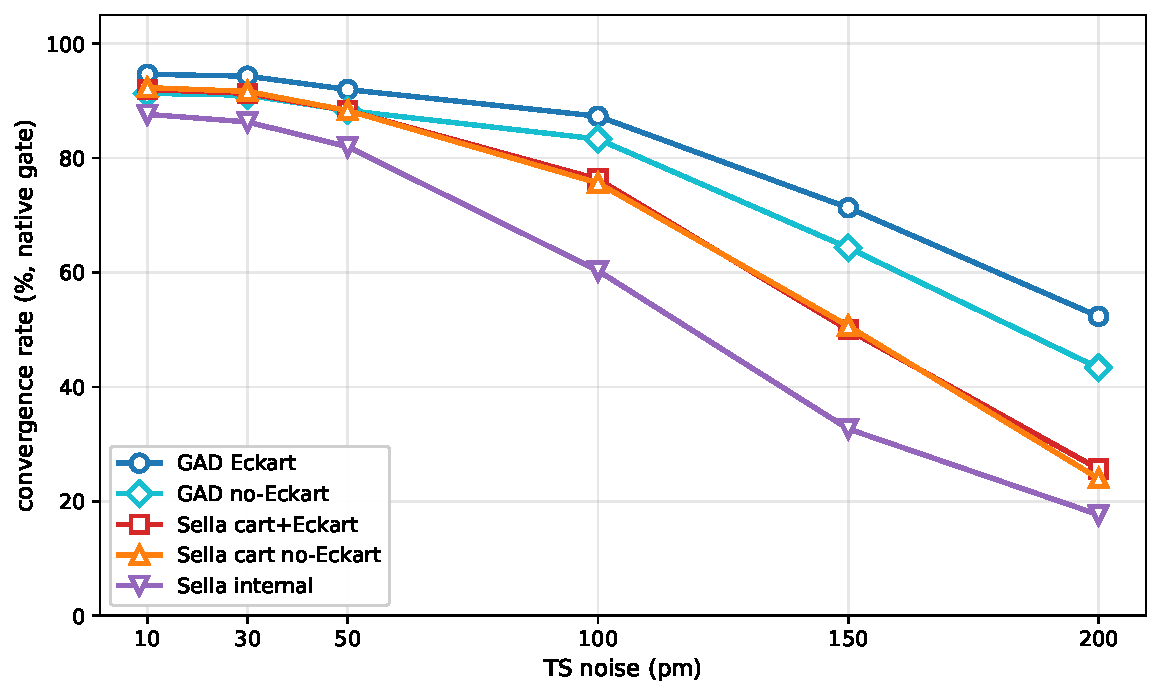
\includegraphics[width=\textwidth]{figures/fig_cmp_conv_5methods.pdf}
\caption{\textbf{Convergence rate (local criterion) vs.\ noise.} Denominator
= 300 samples per cell. Each method uses its native force criterion
(Table in §1.2).}
\label{fig:cmp_conv}
\end{subfigure}
\hfill
\begin{subfigure}[t]{0.495\textwidth}
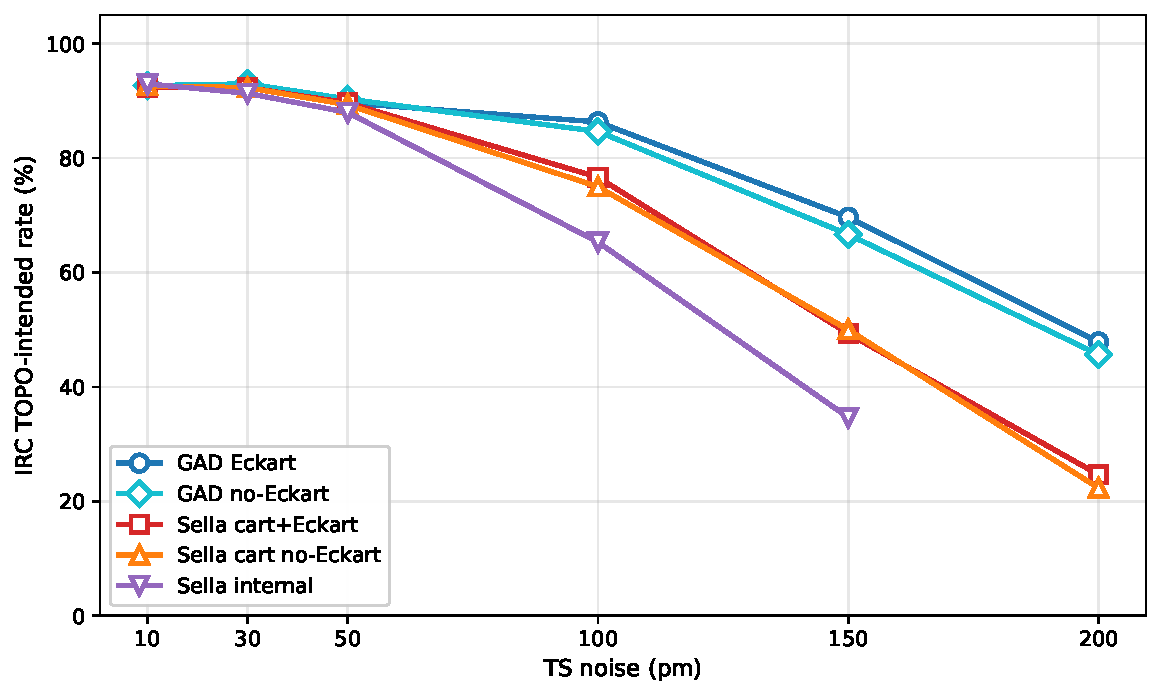
\includegraphics[width=\textwidth]{figures/fig_cmp_irc_topo_5methods.pdf}
\caption{\textbf{IRC TOPO-intended vs.\ noise.} Same 300-sample
denominator. \texttt{sella\_hip} IRC on the final geometry of every
method (converged or not), scored by bond-graph isomorphism against
labeled (R, P).}
\label{fig:cmp_irc}
\end{subfigure}
\caption{\textbf{Ranking is preserved across noise under both local criterion
and IRC.} GAD (blue/cyan) $>$ Sella Cartesian (red/orange) $>$ Sella
internal (purple), with gaps widening at high noise.
The Eckart $\leftrightarrow$ no-Eckart pairs (GAD blue vs.\ cyan; Sella red vs.\ orange)
are essentially on top of each other at low noise and separate only
modestly at 150/200\,pm.}
\label{fig:main_cmp}
\end{figure}

\begin{center}
\textbf{Convergence rate (matched $f_{\max}{<}0.01$ criterion, \% of 300)} \\[0.3em]
\begin{tabular}{l|cccccc}
\toprule
Method & 10\,pm & 30\,pm & 50\,pm & 100\,pm & 150\,pm & 200\,pm \\
\midrule
GAD Eckart fmax (canonical)   & 87.3 & 87.3 & 85.3 & \textbf{80.0} & \textbf{63.7} & \textbf{45.3} \\
GAD no-Eckart                 & 91.3 & 91.0 & 88.3 & 83.3 & 64.3 & 43.3 \\
Sella cart$+$Eckart           & 92.0 & 91.3 & 88.3 & 76.3 & 50.0 & 25.7 \\
Sella cart no-Eckart          & \textbf{92.3} & \textbf{91.7} & \textbf{88.3} & 75.7 & 50.7 & 24.0 \\
Sella internal                & 87.7 & 86.3 & 82.0 & 60.3 & 32.7 & 17.0 \\
\bottomrule
\end{tabular}
\vskip0.8em
\textbf{IRC TOPO-intended (\% of 300)} \\[0.3em]
\begin{tabular}{l|cccccc}
\toprule
Method & 10\,pm & 30\,pm & 50\,pm & 100\,pm & 150\,pm & 200\,pm \\
\midrule
GAD Eckart fmax (canonical)   & \textbf{93.0} & \textbf{93.0} & \textbf{90.7} & \textbf{86.7} & \textbf{70.0} & \textbf{47.0} \\
GAD no-Eckart                 & 92.7 & \textbf{93.0} & 90.3 & 84.7 & 66.7 & 45.7 \\
Sella cart$+$Eckart           & 92.3 & 92.3 & 89.7 & 76.7 & 49.3 & 24.7 \\
Sella cart no-Eckart          & 92.7 & 92.3 & 89.3 & 75.0 & 50.0 & 22.3 \\
Sella internal                & \textbf{93.0} & 91.3 & 88.0 & 65.3 & 34.7 & 18.7 \\
\bottomrule
\end{tabular}
\end{center}

\textbf{Crossover narrative (under matched fmax).} At low noise (10--50\,pm)
the four ``healthy'' methods (GAD Eckart, GAD no-Eckart, Sella cart$\pm$Eckart)
all sit at 85--92\% TS-finding and 90--93\% IRC TOPO --- statistically tied,
with Sella Cartesian holding a $\sim$4\,pp edge in TS-finding (faster QN
convergence on near-saddle starting geometries). At 100\,pm the
ranking flips: GAD pulls ahead by $\sim$5\,pp; by 200\,pm the gap is
$\sim$20\,pp. \textbf{The crossover is at $\sim$75--100\,pm.}

\paragraph{Observation 1: IRC rescues a handful of non-converged samples
for GAD.} At high noise GAD Eckart's IRC TOPO (86.3\% at 100\,pm, 69.7\%
at 150\,pm) is very close to its local-criterion convergence (87.3\% and
71.3\%). Some samples that GAD considered ``not converged'' were in fact
near-TSs whose IRC still validated; others that GAD accepted by the local criterion were
valid-but-wrong minima. Net effect: IRC rate is within 2\,pp of local
criterion.

\paragraph{Observation 2: Sella's IRC rate drops \emph{below} its local
criterion at mid-high noise.} At 100\,pm Sella cart+Eckart has local criterion
76.3\% but IRC TOPO only 76.7\% (essentially equal). At 200\,pm: criterion
25.7\% vs IRC 24.7\%. Sella's failures are ``genuinely stuck'' —
not near a valid TS. This was already flagged in the 2026-04-17 analysis
and is confirmed across all 2000-step Sella variants.

\paragraph{Observation 3: Eckart matters much less than Round~1 reported.}
Under the 2000-step budget, GAD no-Eckart TOPO is \emph{identical} to GAD
Eckart at 10/30\,pm (92.7\% each), and within 3\,pp at every other noise
level. The ``Eckart is the main unlock'' story from Round~1 was dominated
by step-budget effects (see §\ref{sec:eckart_deep}).

\newpage
\clearpage
\subsection{Per-method breakdown: local criterion + IRC side-by-side}

For each method we show the raw convergence-rate line chart (method's
native criterion) next to the IRC-TOPO proportional stacked bar chart
(intended / half / unintended). Denominator is always 300 samples per
noise cell (\emph{not} converged-only).

\begin{figure}[H]
\centering
\begin{subfigure}[t]{0.495\textwidth}
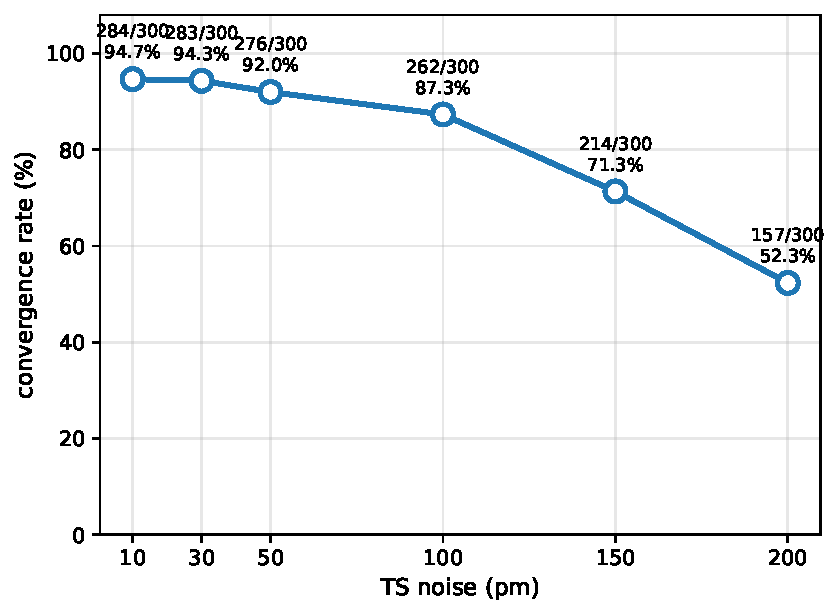
\includegraphics[width=\textwidth]{figures/fig_method_gad_eckart_conv_line.pdf}
\caption{GAD Eckart --- local criterion \\($n_{\text{neg}}{=}1 \wedge \|\mathbf{F}\|_{\text{mean}}{<}0.01$)}
\end{subfigure}
\hfill
\begin{subfigure}[t]{0.495\textwidth}
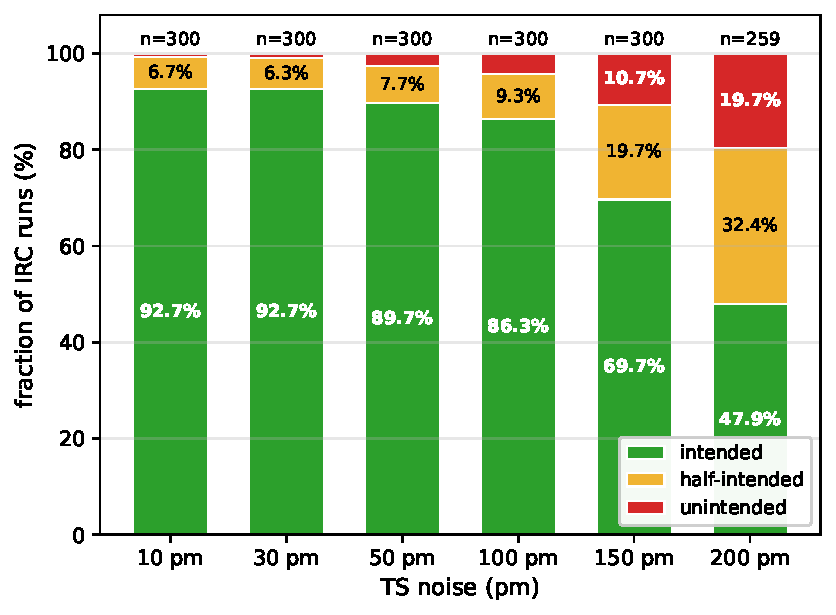
\includegraphics[width=\textwidth]{figures/fig_method_gad_eckart_irc_bars_topo.pdf}
\caption{GAD Eckart --- IRC TOPO (all endpoints)}
\end{subfigure}
\caption{\textbf{\texttt{gad\_dt003} with Eckart projection, dt=0.003, 2000 steps.}
Left: local-criterion convergence rate.
Right: \texttt{sella\_hip} IRC TOPO outcome on every sample's final geometry.
Labels on bars are percentages of the 300-sample universe.}
\end{figure}

\begin{figure}[H]
\centering
\begin{subfigure}[t]{0.495\textwidth}
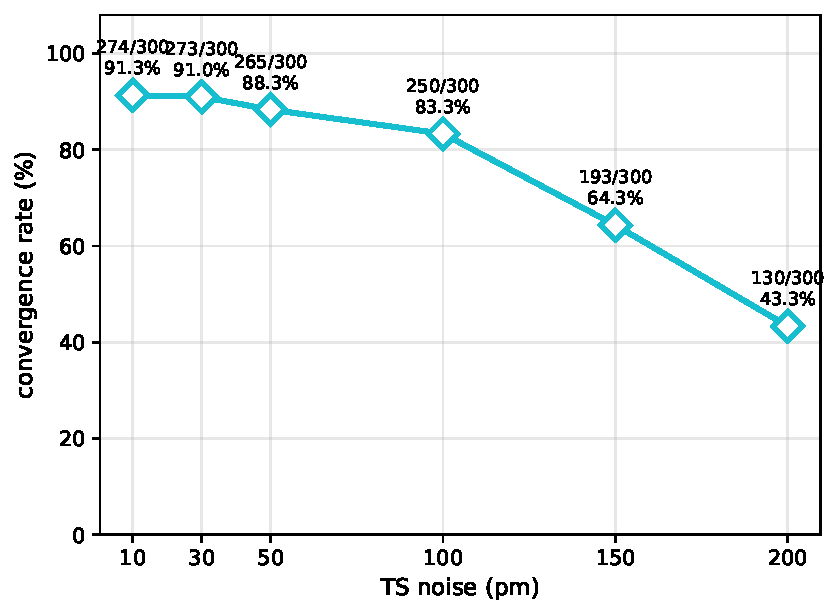
\includegraphics[width=\textwidth]{figures/fig_method_gad_no_eckart_conv_line.pdf}
\caption{GAD no-Eckart --- local criterion \\($n_{\text{neg}}{=}1 \wedge f_{\max}{<}0.01$)}
\end{subfigure}
\hfill
\begin{subfigure}[t]{0.495\textwidth}
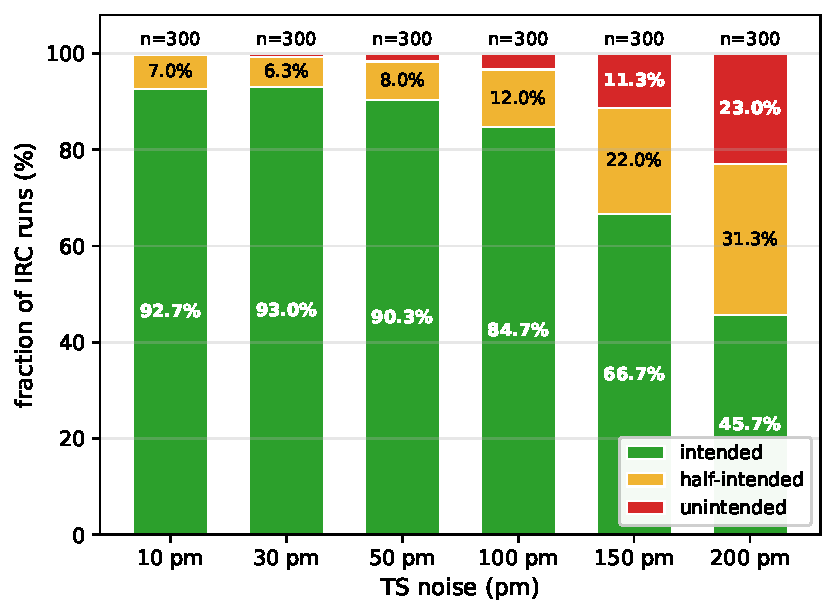
\includegraphics[width=\textwidth]{figures/fig_method_gad_no_eckart_irc_bars_topo.pdf}
\caption{GAD no-Eckart --- IRC TOPO (all endpoints)}
\end{subfigure}
\caption{\textbf{\texttt{gad\_dt003\_no\_eckart}: raw Hessian GAD, dt=0.003, 2000 steps.}
Eckart projection removed from dynamics; local criterion uses fmax.}
\end{figure}

\begin{figure}[H]
\centering
\begin{subfigure}[t]{0.495\textwidth}
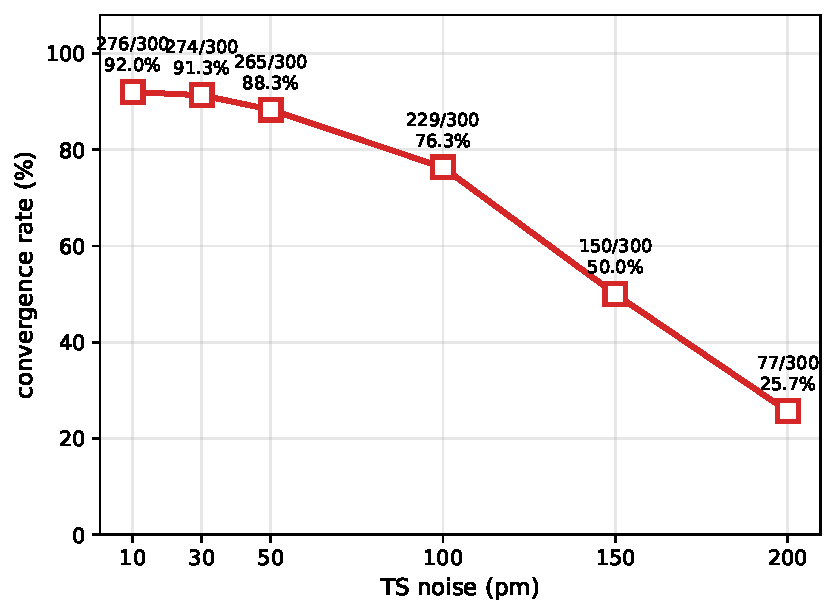
\includegraphics[width=\textwidth]{figures/fig_method_sella_carte_2k_conv_line.pdf}
\caption{Sella cart+Eckart --- local criterion \\($n_{\text{neg}}{=}1 \wedge f_{\max}{<}0.01$)}
\end{subfigure}
\hfill
\begin{subfigure}[t]{0.495\textwidth}
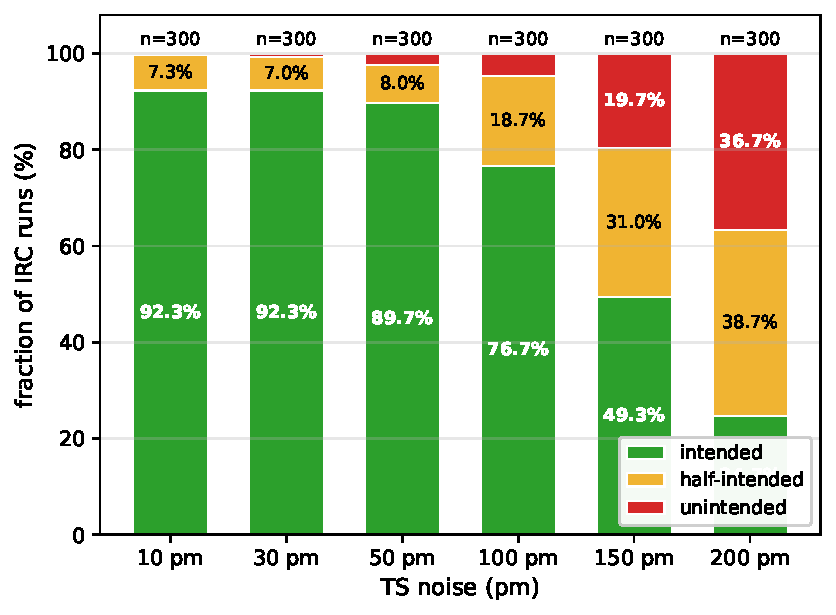
\includegraphics[width=\textwidth]{figures/fig_method_sella_carte_2k_irc_bars_topo.pdf}
\caption{Sella cart+Eckart --- IRC TOPO (all endpoints)}
\end{subfigure}
\caption{\textbf{Sella cartesian + Eckart, 2000 steps, HIP Hessian every step.}}
\end{figure}

\begin{figure}[H]
\centering
\begin{subfigure}[t]{0.495\textwidth}
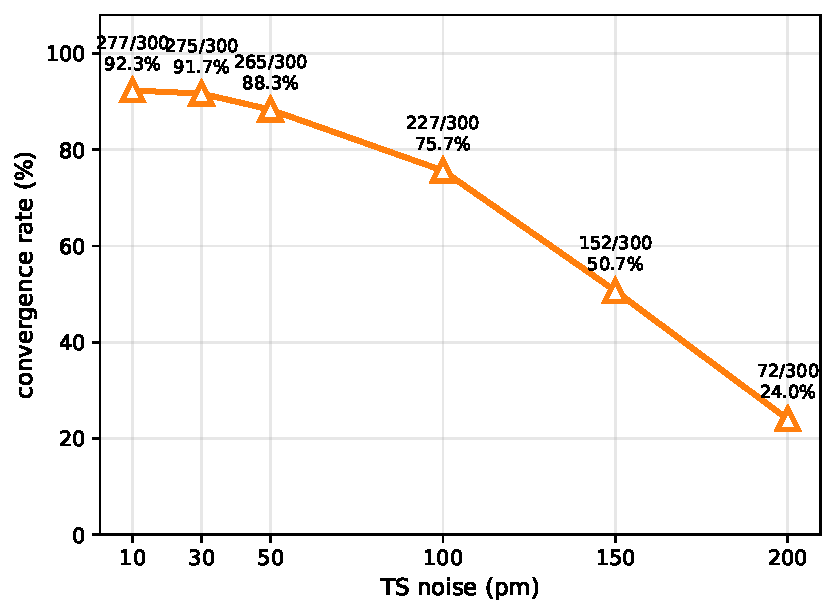
\includegraphics[width=\textwidth]{figures/fig_method_sella_cart_2k_conv_line.pdf}
\caption{Sella cart no-Eckart --- local criterion}
\end{subfigure}
\hfill
\begin{subfigure}[t]{0.495\textwidth}
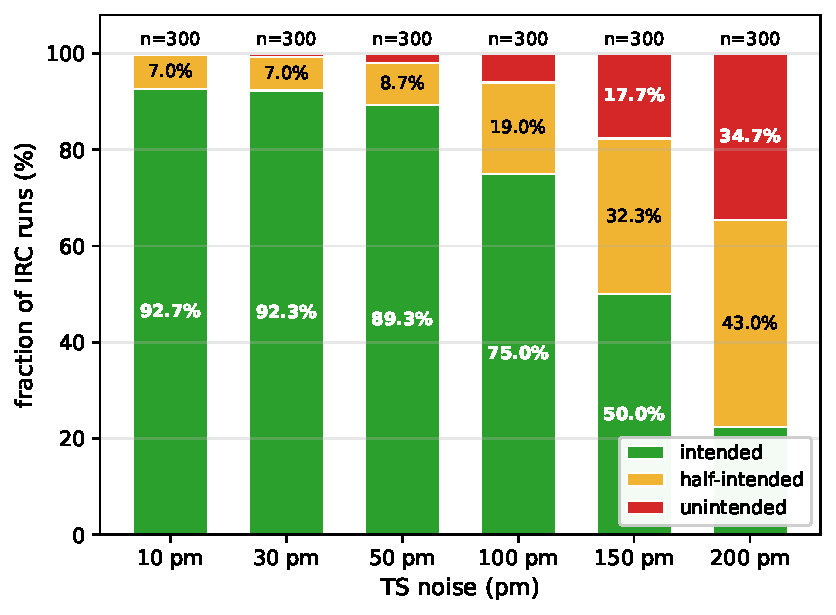
\includegraphics[width=\textwidth]{figures/fig_method_sella_cart_2k_irc_bars_topo.pdf}
\caption{Sella cart no-Eckart --- IRC TOPO (all endpoints)}
\end{subfigure}
\caption{\textbf{Sella cartesian, no Eckart, 2000 steps, HIP Hessian every step.}}
\end{figure}

\begin{figure}[H]
\centering
\begin{subfigure}[t]{0.495\textwidth}
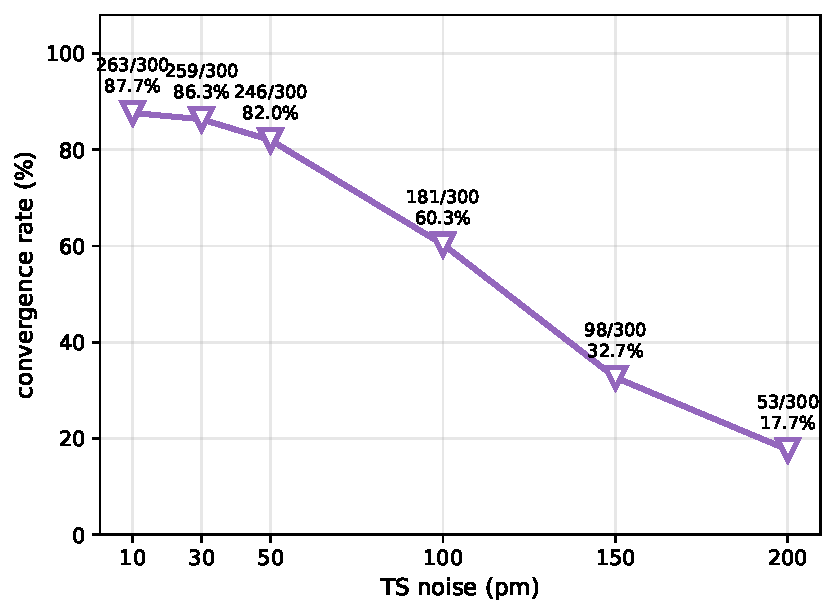
\includegraphics[width=\textwidth]{figures/fig_method_sella_int_2k_conv_line.pdf}
\caption{Sella internal --- local criterion}
\end{subfigure}
\hfill
\begin{subfigure}[t]{0.495\textwidth}
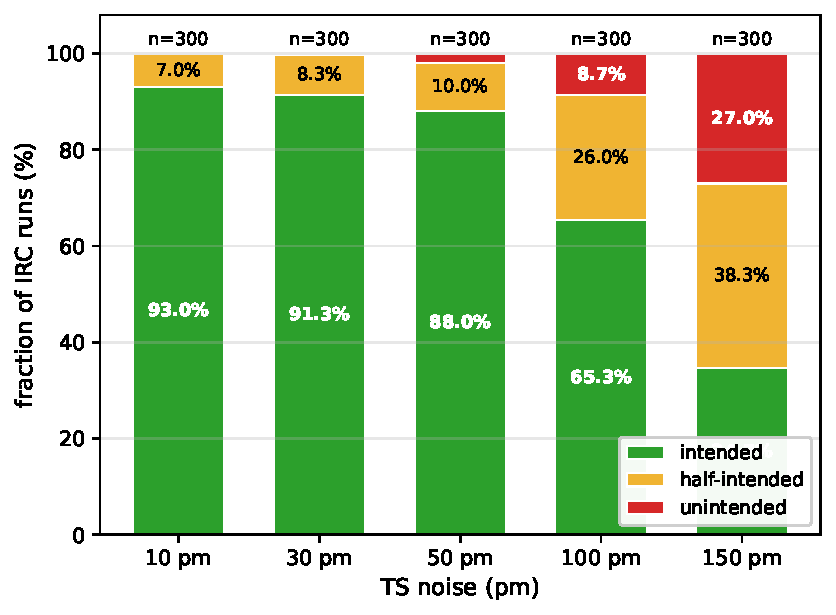
\includegraphics[width=\textwidth]{figures/fig_method_sella_int_2k_irc_bars_topo.pdf}
\caption{Sella internal --- IRC TOPO (all endpoints)}
\end{subfigure}
\caption{\textbf{Sella internal coords (no Eckart --- Sella handles DOF removal
intrinsically), 2000 steps, HIP Hessian every step.}
200\,pm IRC cell still computing at report time.}
\end{figure}

\newpage
\clearpage
% =================================================================
\section{Eckart vs no-Eckart --- Brief Note (full deep-dive in Appendix)}
\label{sec:eckart_brief}
% =================================================================

The original Round~1 result was ``Eckart projection is the main unlock
for GAD''. We re-examined this carefully under the matched
$f_{\max}{<}0.01$ criterion; both ``unlock'' and the previously-reported
``$1.33\times$ step efficiency'' \textbf{do not survive the corrected
analysis}.

\begin{center}
\textbf{Same-sample step efficiency, matched fmax criterion.} \\[0.3em]
\begin{tabular}{rcccc}
\toprule
Noise & $n$ shared & Eckart median steps & no-Eckart median steps & ratio (N/E) \\
\midrule
10\,pm  & 261 & 137 & 124 & 0.91$\times$ \\
30\,pm  & 261 & 290 & 263 & 0.91$\times$ \\
50\,pm  & 254 & 406 & 380 & 0.94$\times$ \\
100\,pm & 236 & 620 & 589 & 0.95$\times$ \\
150\,pm & 171 & 771 & 742 & 0.96$\times$ \\
200\,pm & 103 & 866 & 839 & 0.97$\times$ \\
\bottomrule
\end{tabular}
\end{center}

\textbf{Eckart is not a step-efficiency multiplier.} Under fair
comparison (both methods using fmax<0.01), no-Eckart is \emph{slightly
faster}: ratio 0.91--0.97$\times$. Convergence rates are within 1--2\,pp
($\pm$1\,pp at low noise, no-Eckart slightly higher actually); IRC-TOPO
agreement is $>$95\% per-sample at low noise. The full deep-dive
(per-sample agreement, IRC outcome correlation, why each method has
unique converged samples at high noise, and the corrected Round~1
explanation) is in Appendix~\ref{sec:eckart_appendix}.

\newpage
\clearpage
% =================================================================
\section{Criterion vs IRC Sample Overlap}
% =================================================================

For each method and noise level, every sample falls into one of four
quadrants: \{local criterion pass, IRC TOPO pass\}. This quantifies whether
a method's ``converged'' label agrees with IRC's verdict.

\begin{figure}[H]
\centering
\begin{subfigure}[t]{0.48\textwidth}
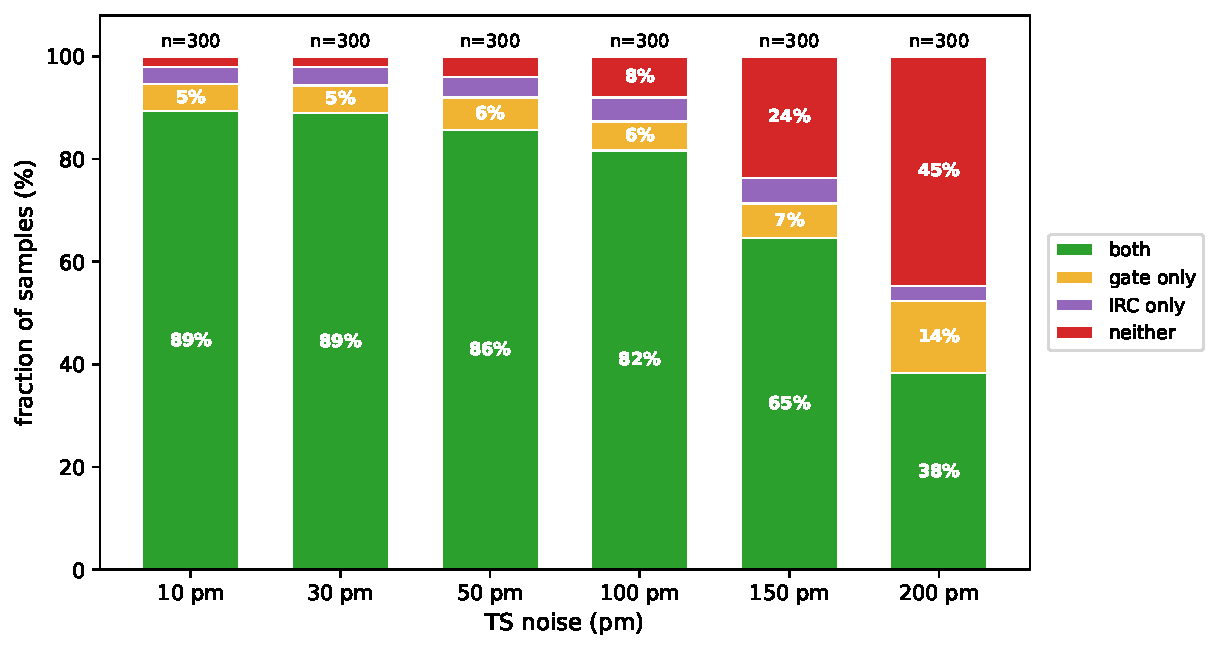
\includegraphics[width=\textwidth]{figures/fig_gate_vs_irc_gad_eckart.pdf}
\caption{GAD Eckart}
\end{subfigure}
\hfill
\begin{subfigure}[t]{0.48\textwidth}
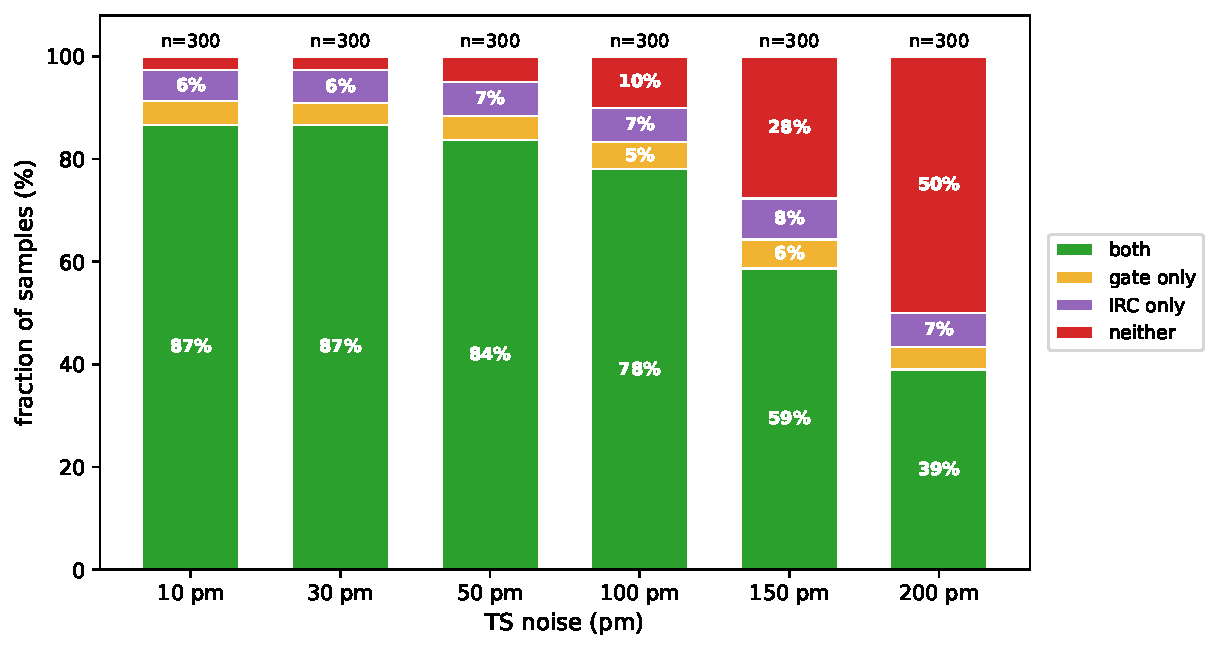
\includegraphics[width=\textwidth]{figures/fig_gate_vs_irc_gad_no_eckart.pdf}
\caption{GAD no-Eckart}
\end{subfigure}
\vskip0.5em
\begin{subfigure}[t]{0.48\textwidth}
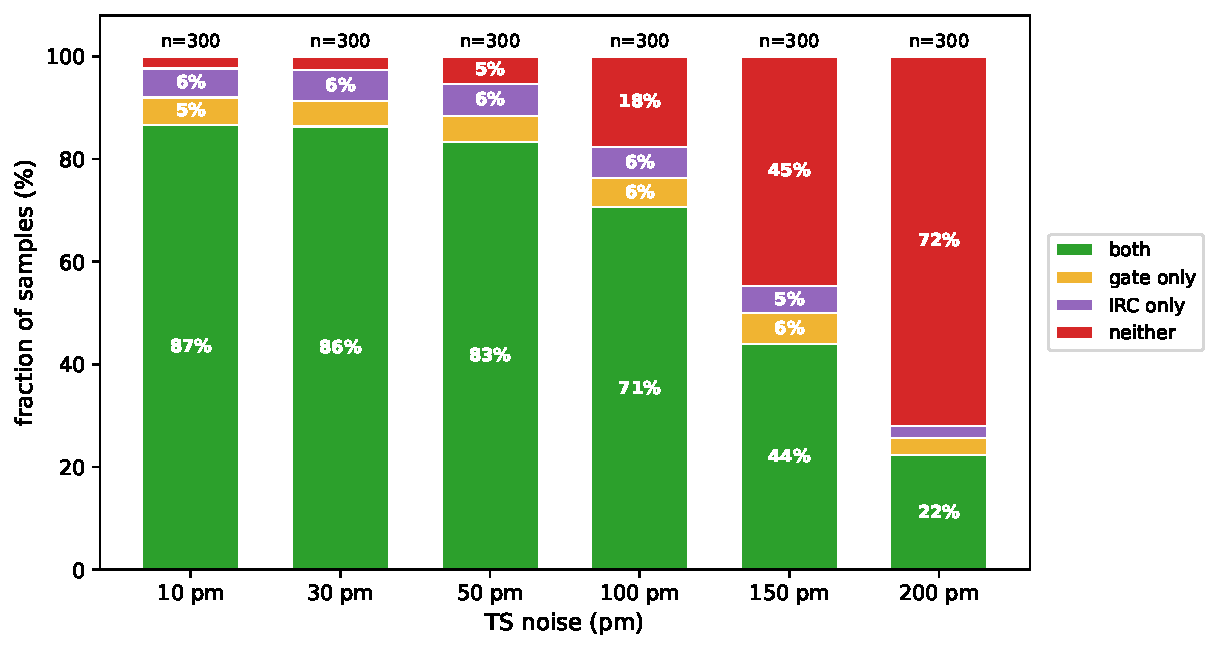
\includegraphics[width=\textwidth]{figures/fig_gate_vs_irc_sella_carte_2k.pdf}
\caption{Sella cart+Eckart}
\end{subfigure}
\hfill
\begin{subfigure}[t]{0.48\textwidth}
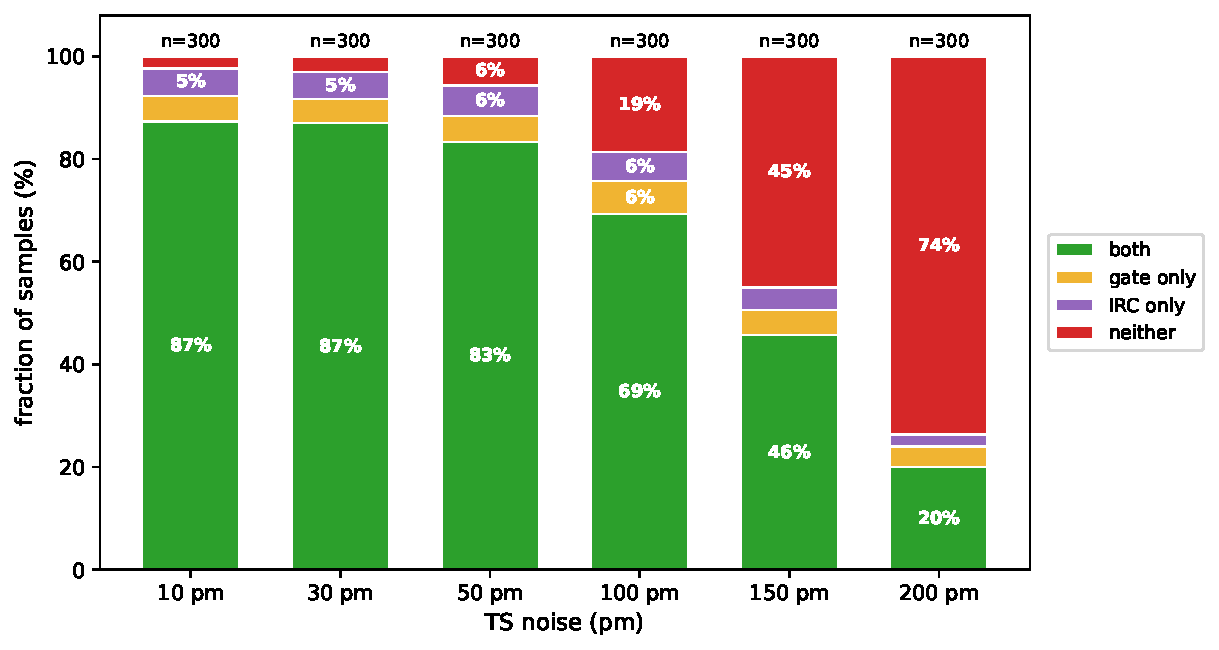
\includegraphics[width=\textwidth]{figures/fig_gate_vs_irc_sella_cart_2k.pdf}
\caption{Sella cart no-Eckart}
\end{subfigure}
\vskip0.5em
\begin{subfigure}[t]{0.48\textwidth}
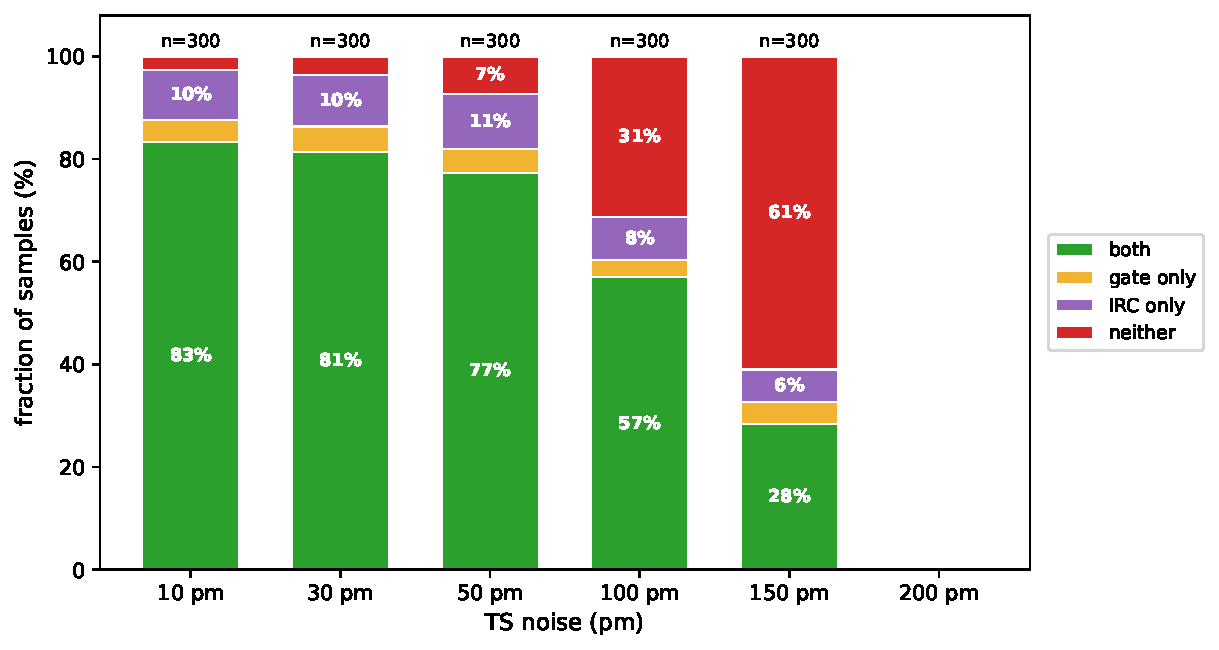
\includegraphics[width=\textwidth]{figures/fig_gate_vs_irc_sella_int_2k.pdf}
\caption{Sella internal}
\end{subfigure}
\caption{\textbf{Per-method criterion vs.\ IRC-TOPO overlap, all 5 methods.}
Green (``both''): criterion-converged AND IRC-TOPO passes. Yellow
(``criterion only''): criterion says converged, IRC disagrees (over-claim by
local criterion). Purple (``IRC only''): criterion says failed, IRC says
chemically correct (under-claim by local criterion). Red (``neither''):
both agree the sample failed. The red region grows sharply with noise
for Sella and internal; stays small for GAD.}
\end{figure}

\newpage
\clearpage
% =================================================================
\section{Compute Costs}
% =================================================================

\begin{center}
\textbf{Median wall time per sample (s)} \\[0.3em]
\begin{tabular}{l|cccccc}
\toprule
Method & 10\,pm & 30\,pm & 50\,pm & 100\,pm & 150\,pm & 200\,pm \\
\midrule
GAD Eckart                  & 3.9 & 7.3 & 13.7 & 23.9 & 51.5 & 86.1 \\
GAD no-Eckart               & 6.9 & 10.3 & 16.5 & 24.9 & 49.5 & 80.0 \\
Sella cart+Eckart           & 2.3 & 3.7 & 6.3 & 16.4 & 58.9 & 113.2 \\
Sella cart no-Eckart        & 2.2 & 3.5 & 6.2 & 17.2 & 55.0 & 119.6 \\
Sella internal              & 4.3 & 5.6 & 10.3 & 46.7 & 117.4 & 151.7 \\
\bottomrule
\end{tabular}
\end{center}

\begin{center}
\textbf{Valid TSs per GPU-hour (local criterion)} \\[0.3em]
\begin{tabular}{l|cccccc}
\toprule
Method & 10\,pm & 30\,pm & 50\,pm & 100\,pm & 150\,pm & 200\,pm \\
\midrule
GAD Eckart                  & 227 & 158 & 115 & 70 & 40 & 22 \\
GAD no-Eckart               & 168 & 115 & 84 & 56 & 30 & 16.5 \\
Sella cart+Eckart           & \textbf{264} & \textbf{249} & \textbf{175} & 79 & 24 & 8.6 \\
Sella cart no-Eckart        & 267 & 252 & 177 & 75 & 26 & 7.7 \\
Sella internal              & 148 & 116 & 84 & 31 & 10 & 4 \\
\bottomrule
\end{tabular}
\end{center}

Crossover is at $\sim$100\,pm. Below: Sella cartesian is fastest source
of valid TSs. Above: GAD --- the Sella convergence-rate collapse
dominates per-hour yield.

\newpage
% =================================================================
\section{Appendix}
% =================================================================

\clearpage
\subsection{Per-method bar charts: RMSD and endpoint vibrational quality}

Three criteria per method: TOPO (already shown in §2.2), strict RMSD
($<0.3$\,\AA), endpoint vibrational quality (both / one / neither at
vibrational minimum).

\begin{figure}[H]
\centering
\begin{subfigure}[t]{0.48\textwidth}
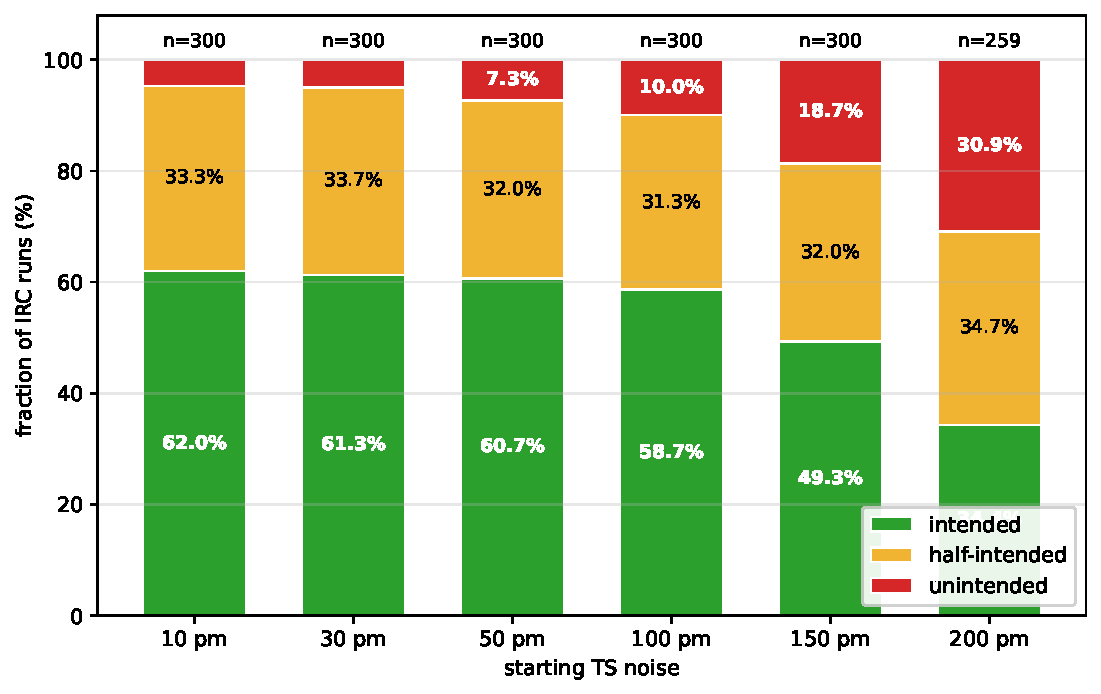
\includegraphics[width=\textwidth]{figures/fig_sella_allep_bars_rmsd.pdf}
\caption{GAD Eckart, RMSD}
\end{subfigure}
\hfill
\begin{subfigure}[t]{0.48\textwidth}
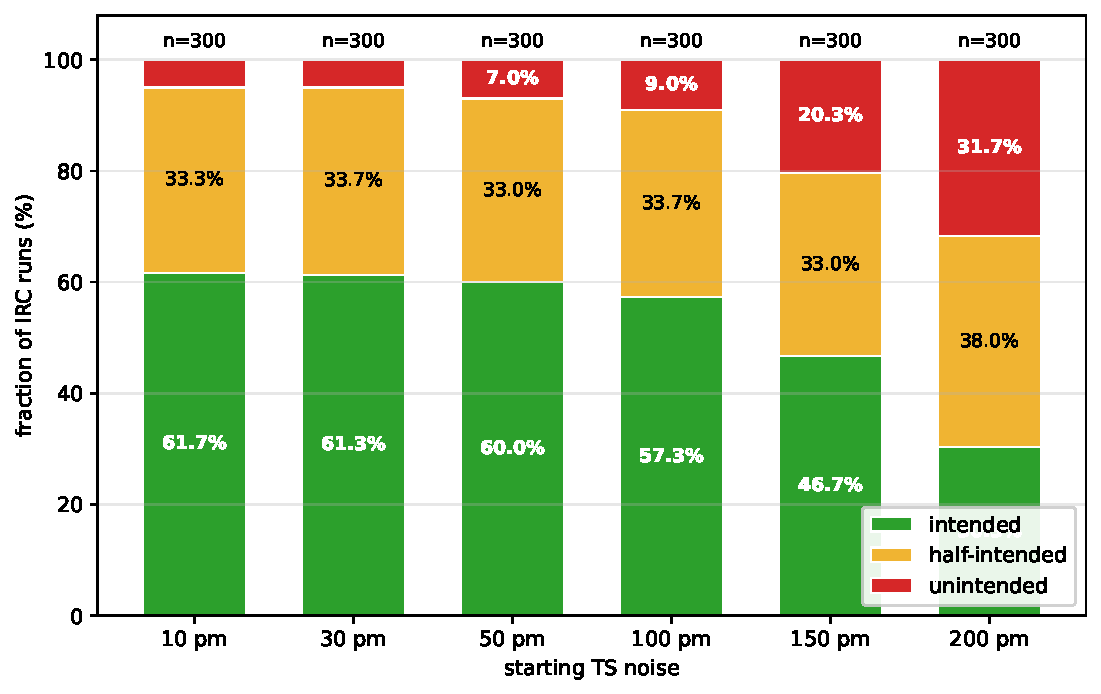
\includegraphics[width=\textwidth]{figures/fig_gad_noeck_new_bars_rmsd.pdf}
\caption{GAD no-Eckart, RMSD}
\end{subfigure}
\vskip0.5em
\begin{subfigure}[t]{0.48\textwidth}
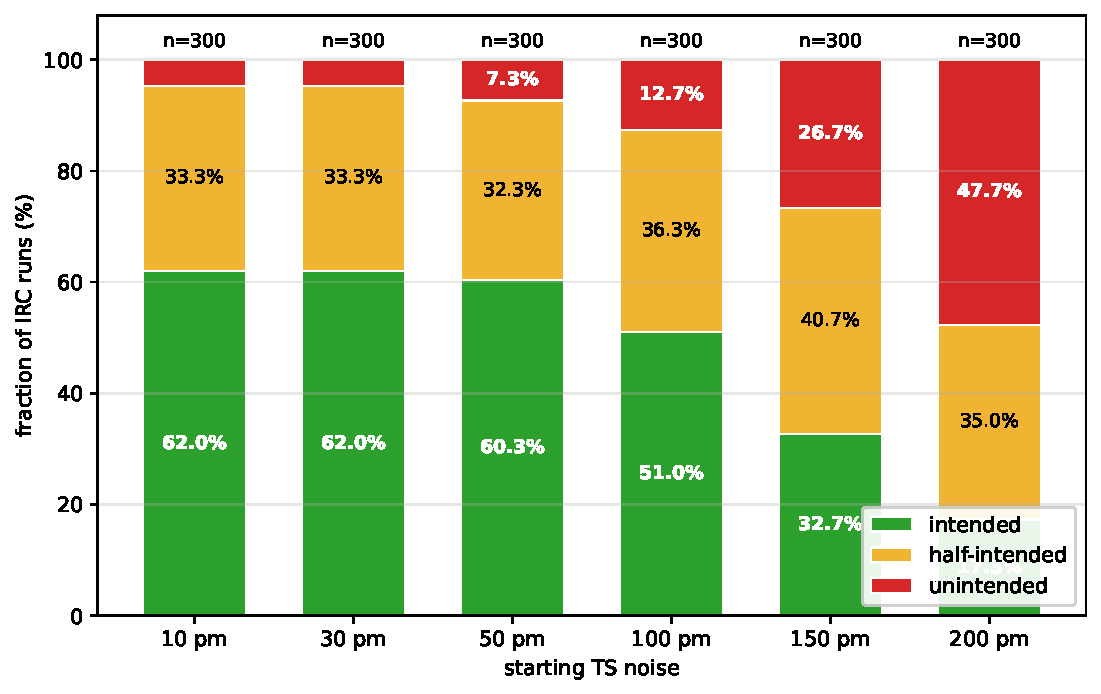
\includegraphics[width=\textwidth]{figures/fig_sella_carte_2k_bars_rmsd.pdf}
\caption{Sella cart+Eckart, RMSD}
\end{subfigure}
\hfill
\begin{subfigure}[t]{0.48\textwidth}
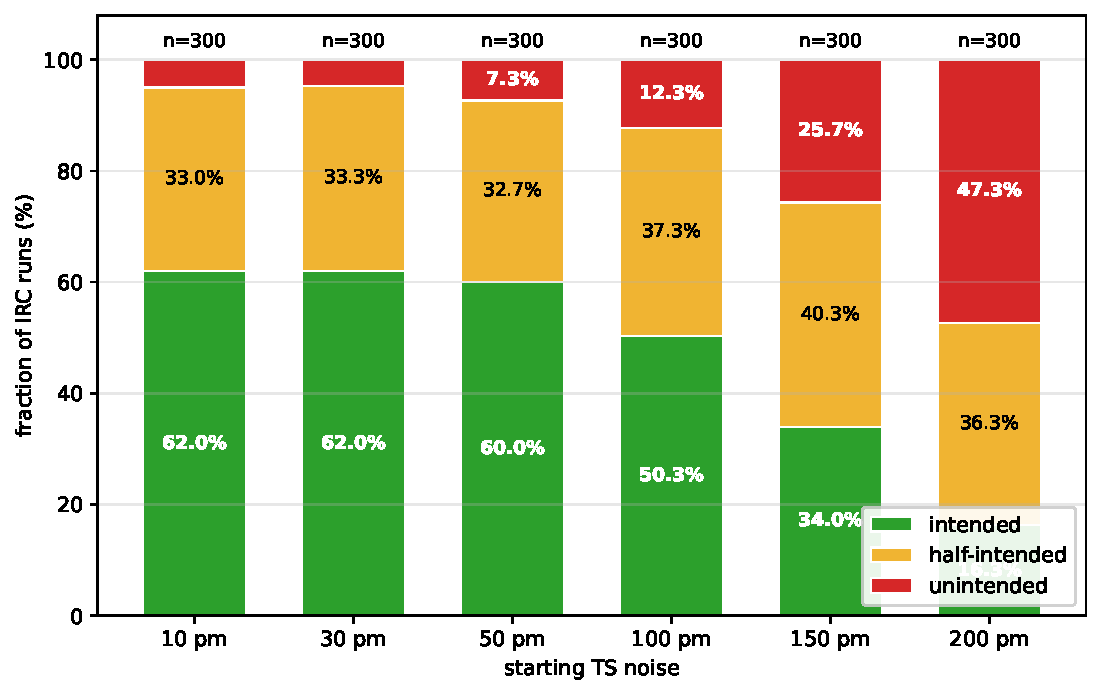
\includegraphics[width=\textwidth]{figures/fig_sella_cart_2k_bars_rmsd.pdf}
\caption{Sella cart no-Eckart, RMSD}
\end{subfigure}
\vskip0.5em
\begin{subfigure}[t]{0.48\textwidth}
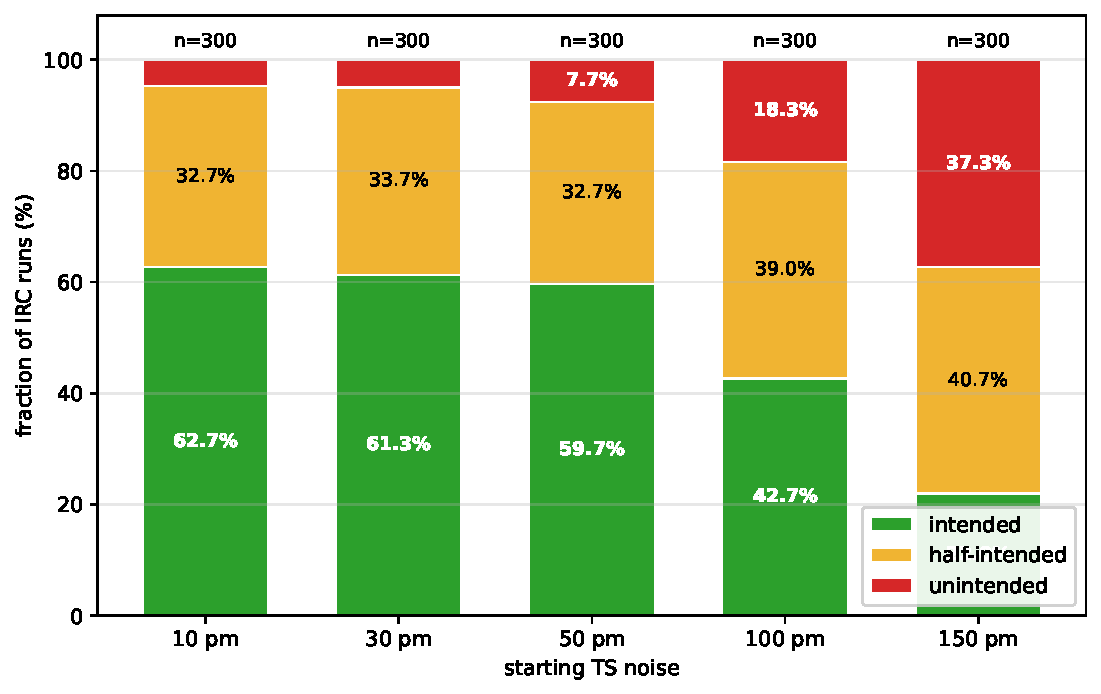
\includegraphics[width=\textwidth]{figures/fig_sella_int_2k_bars_rmsd.pdf}
\caption{Sella internal, RMSD}
\end{subfigure}
\caption{\textbf{Strict RMSD criterion ($<0.3$\,\AA) per method.}
Denominator = 300 samples per cell.}
\end{figure}

\begin{figure}[H]
\centering
\begin{subfigure}[t]{0.48\textwidth}
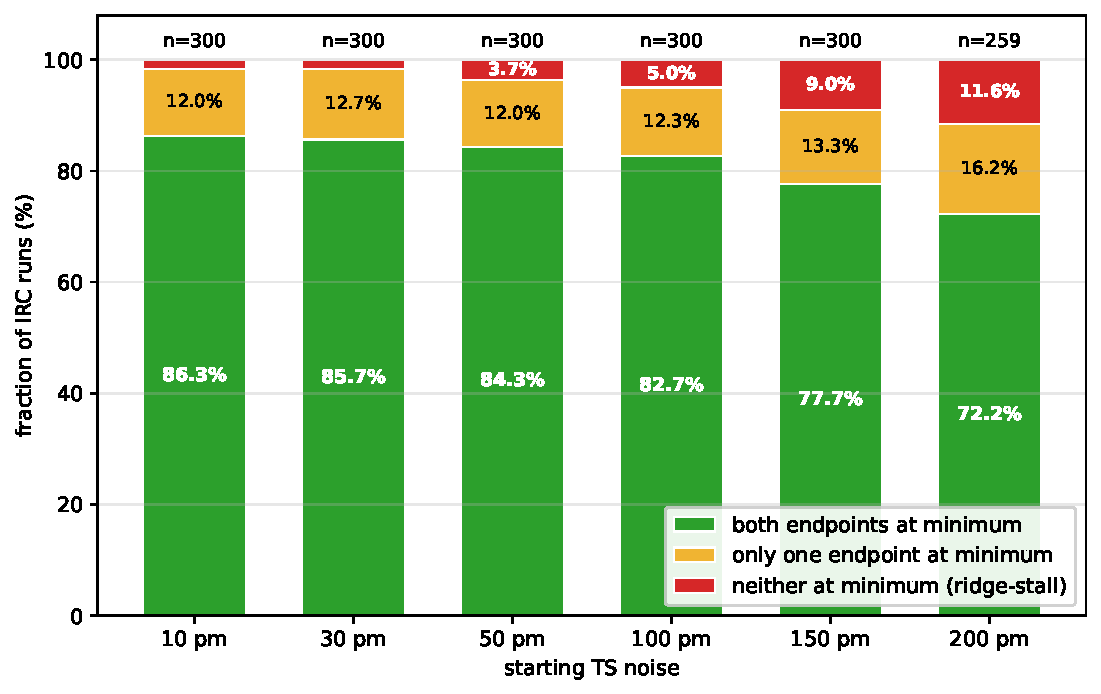
\includegraphics[width=\textwidth]{figures/fig_sella_allep_bars_endpoint.pdf}
\caption{GAD Eckart}
\end{subfigure}
\hfill
\begin{subfigure}[t]{0.48\textwidth}
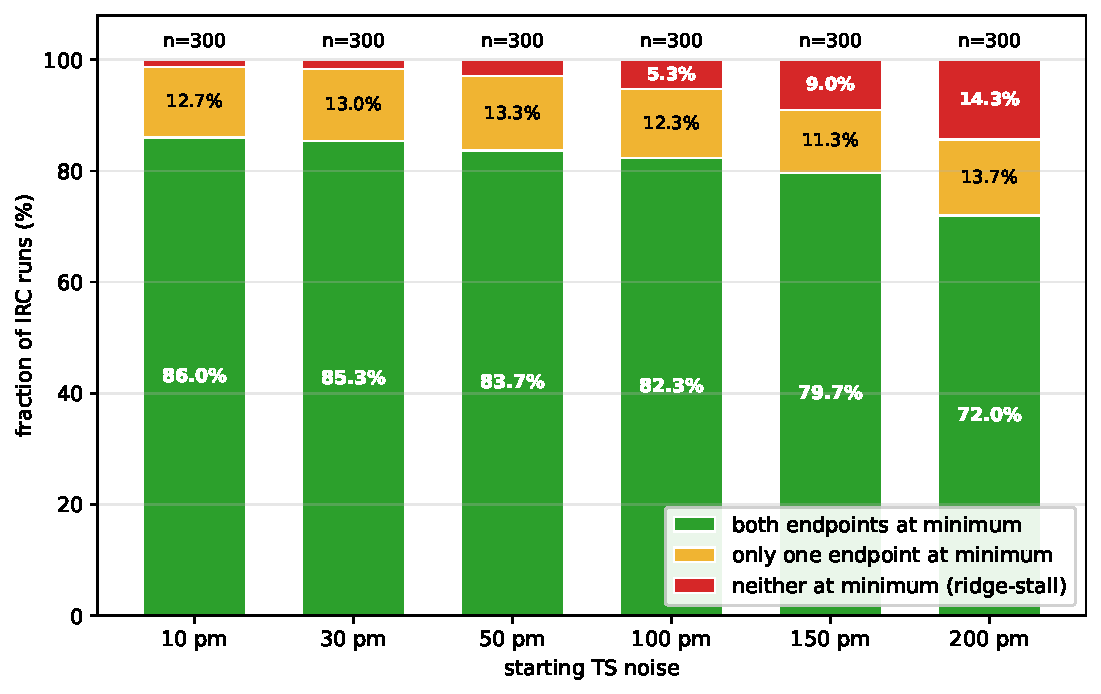
\includegraphics[width=\textwidth]{figures/fig_gad_noeck_new_bars_endpoint.pdf}
\caption{GAD no-Eckart}
\end{subfigure}
\vskip0.5em
\begin{subfigure}[t]{0.48\textwidth}
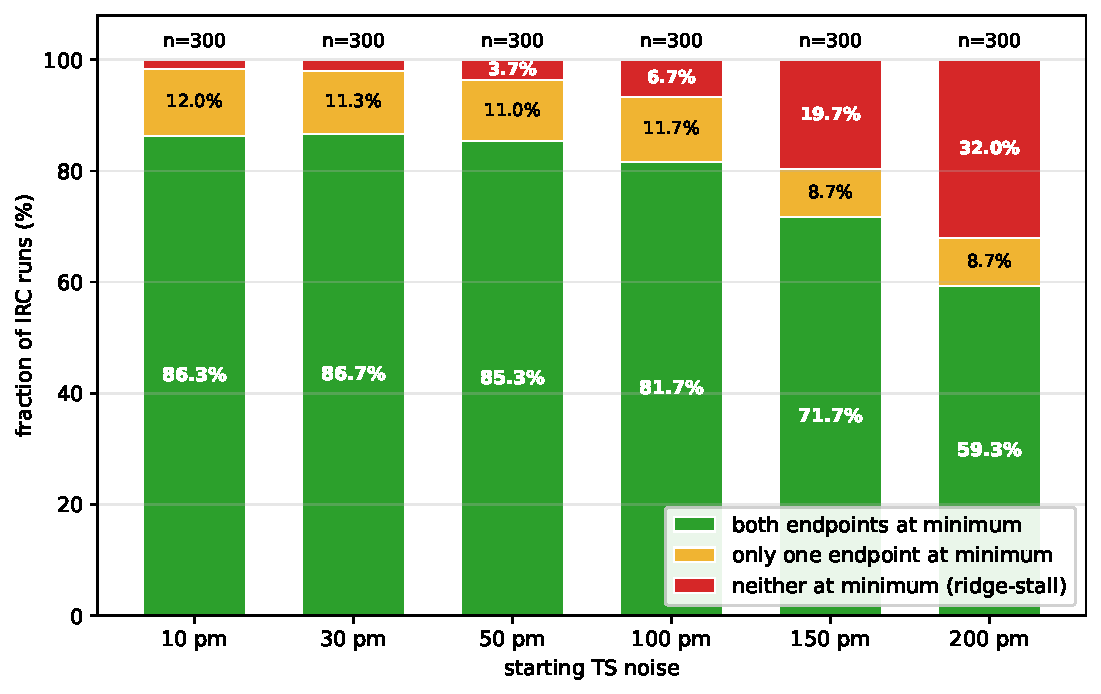
\includegraphics[width=\textwidth]{figures/fig_sella_carte_2k_bars_endpoint.pdf}
\caption{Sella cart+Eckart}
\end{subfigure}
\hfill
\begin{subfigure}[t]{0.48\textwidth}
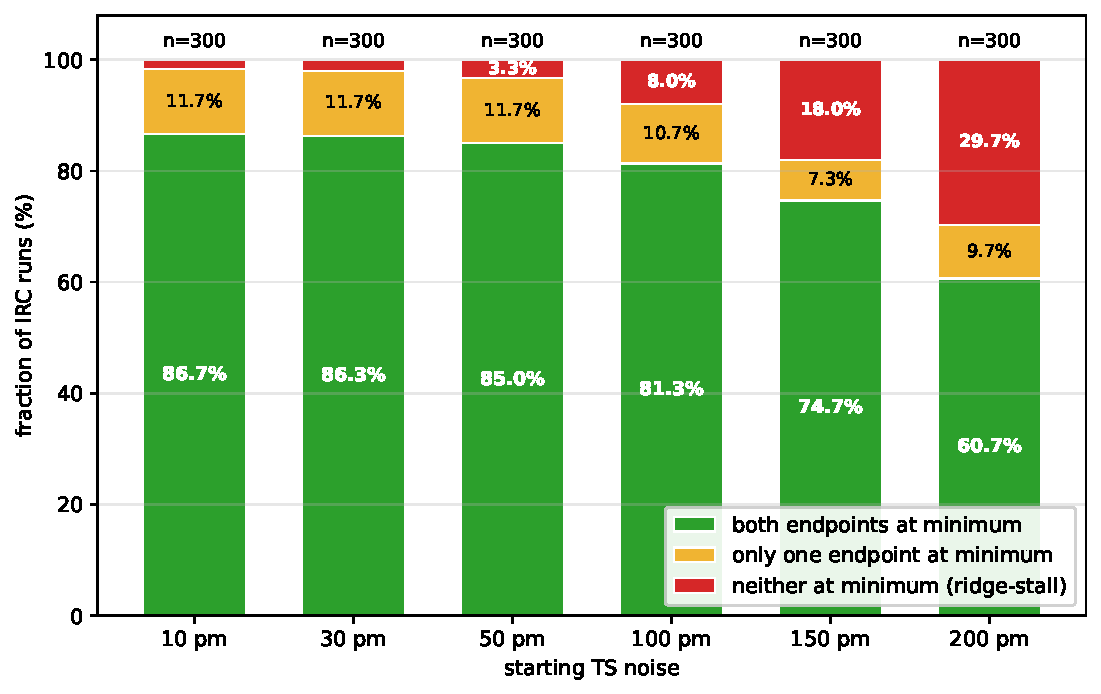
\includegraphics[width=\textwidth]{figures/fig_sella_cart_2k_bars_endpoint.pdf}
\caption{Sella cart no-Eckart}
\end{subfigure}
\vskip0.5em
\begin{subfigure}[t]{0.48\textwidth}
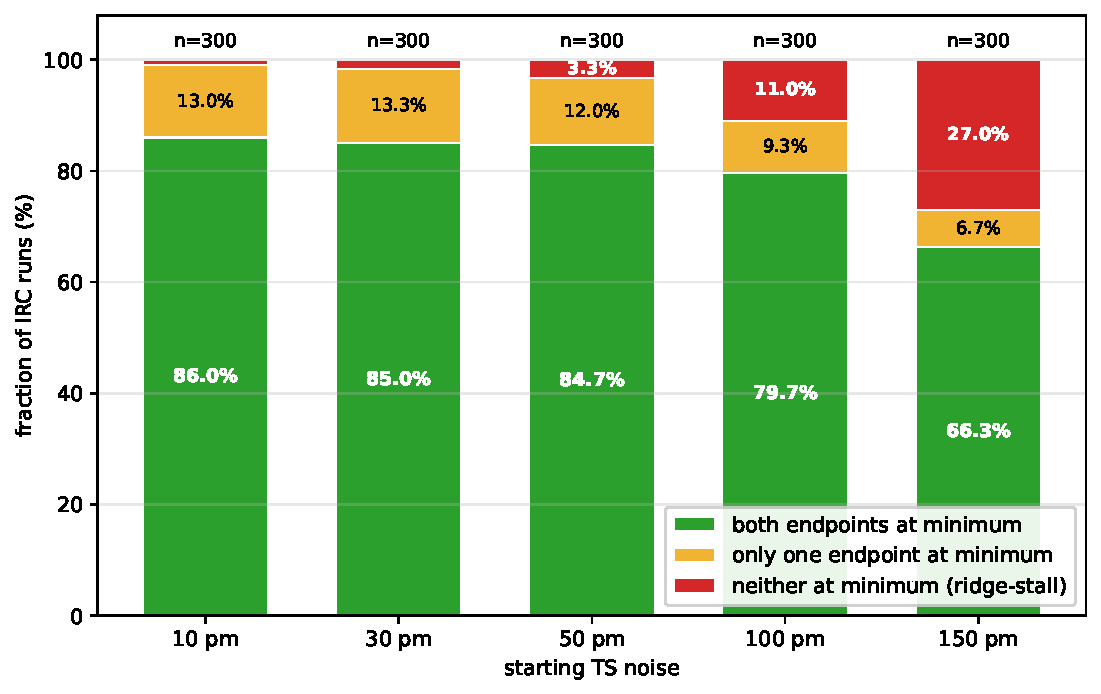
\includegraphics[width=\textwidth]{figures/fig_sella_int_2k_bars_endpoint.pdf}
\caption{Sella internal}
\end{subfigure}
\caption{\textbf{Endpoint vibrational quality per method.} Both / one /
neither IRC endpoint reaches a true minimum
($n_{\text{neg,vib}}{=}0$ on Eckart-projected Hessian).}
\end{figure}

\newpage
\clearpage
\subsection{All-three-classes line charts (cluttered, appendix only)}

The main narrative uses ``intended only'' lines for readability. For
completeness, the ``intended + half + unintended'' breakdown per method:

\begin{figure}[H]
\centering
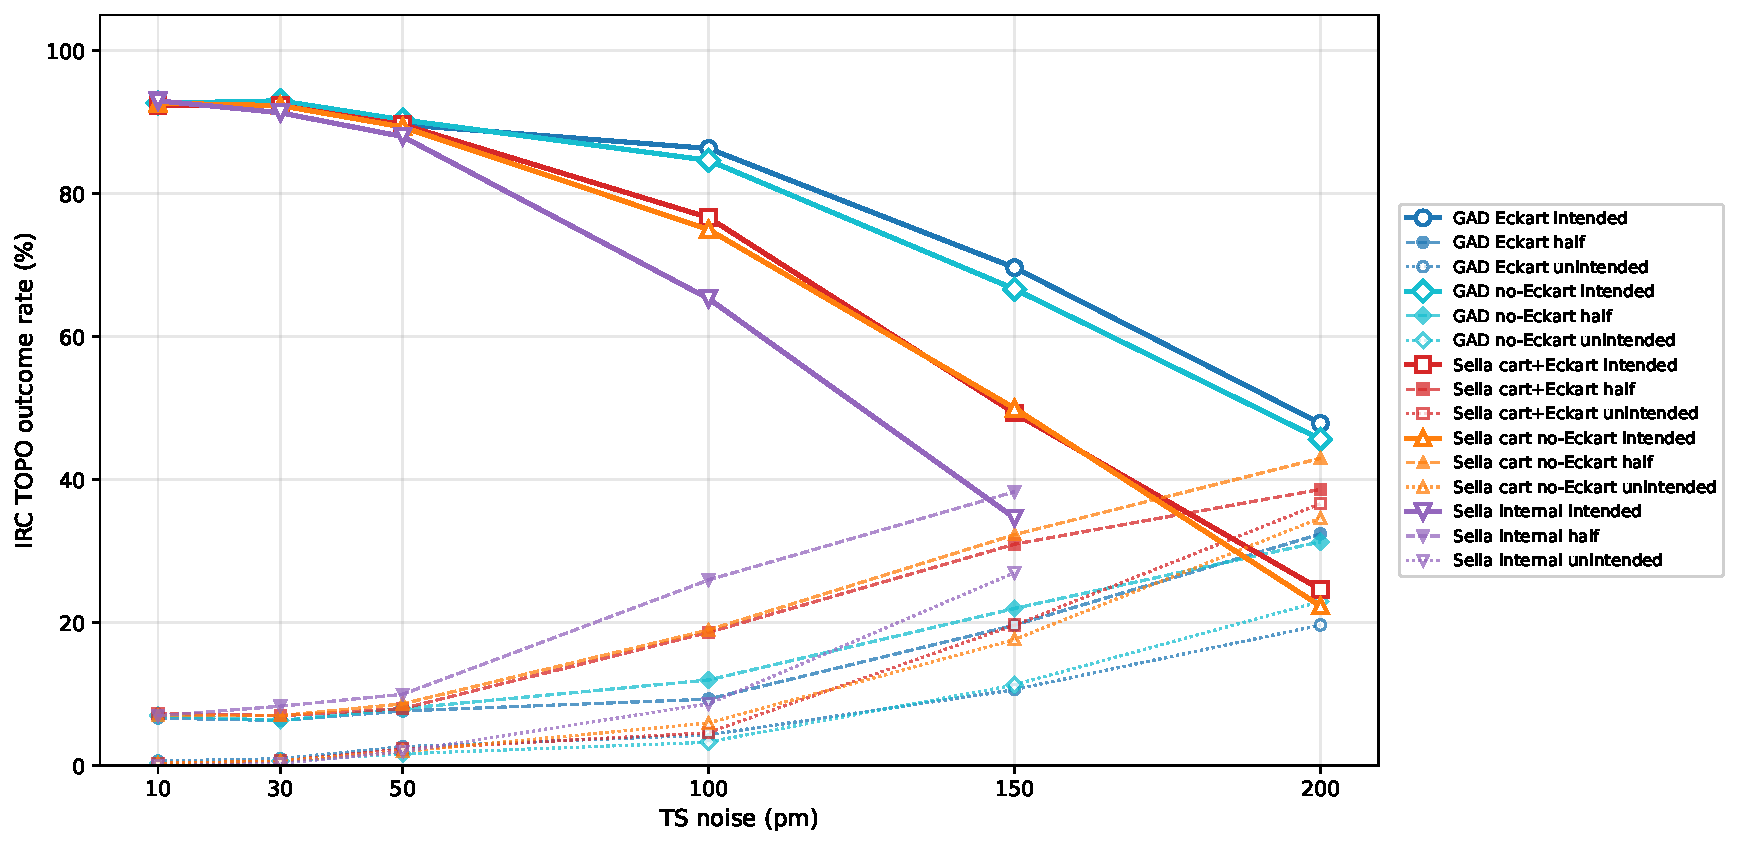
\includegraphics[width=0.95\textwidth]{figures/fig_cmp_irc_topo_all_classes_5methods.pdf}
\caption{\textbf{IRC TOPO outcomes --- all three classes, all five
methods.} 15 lines total: solid = intended, dashed = half-intended,
dotted = unintended. Cluttered on purpose; see §2.1 for the uncluttered
headline view.}
\end{figure}

\begin{figure}[H]
\centering
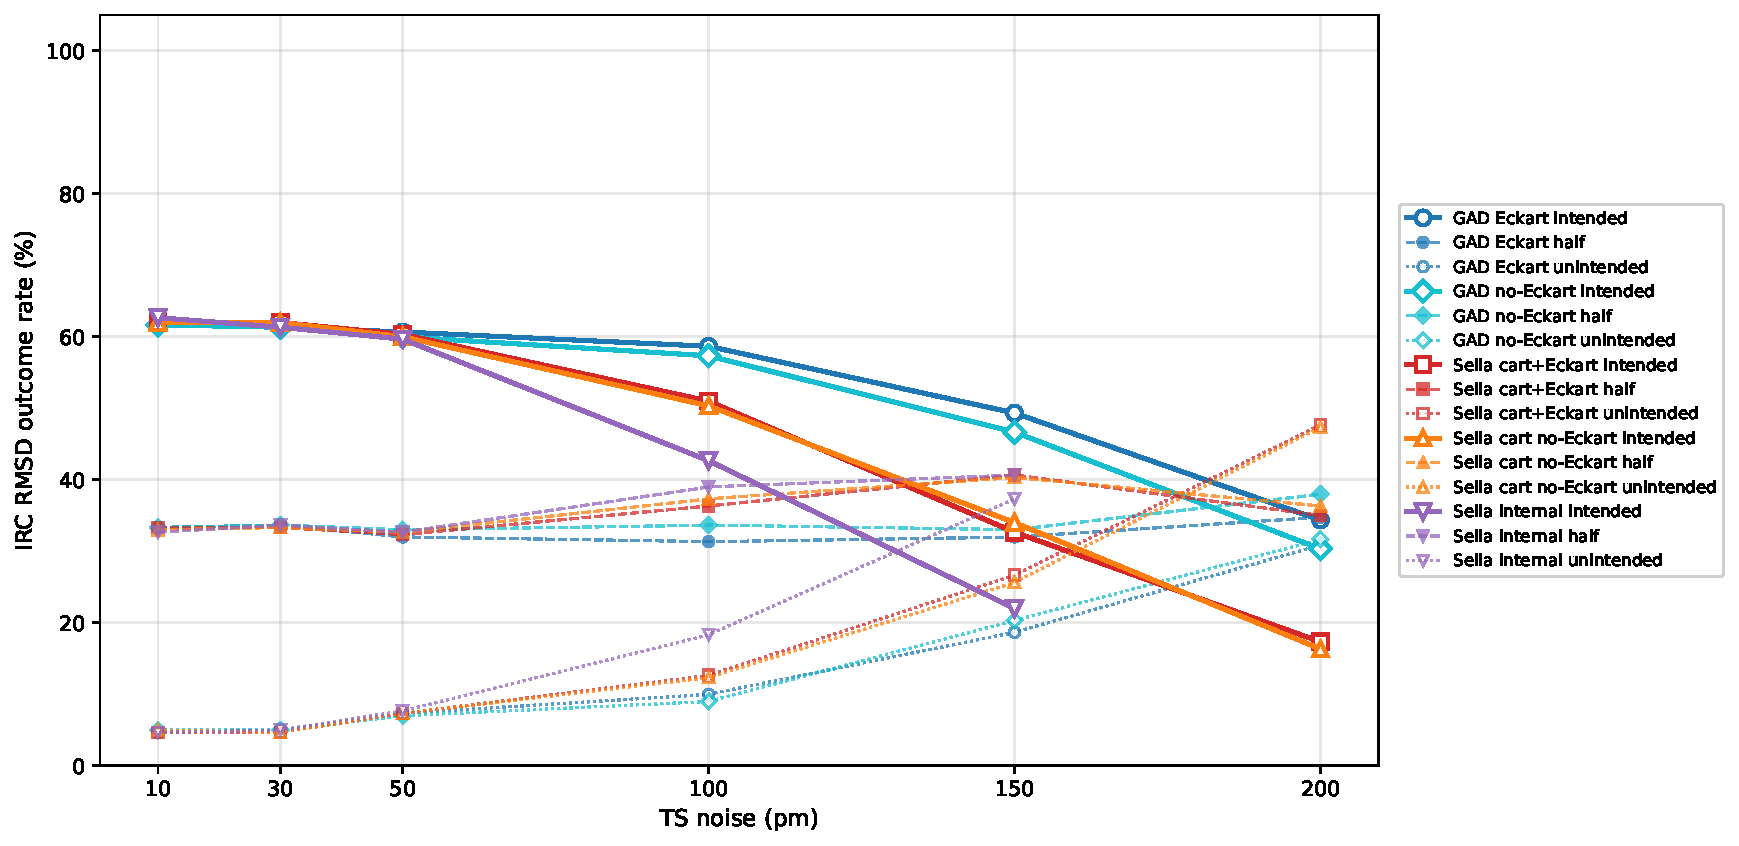
\includegraphics[width=0.95\textwidth]{figures/fig_cmp_irc_rmsd_all_classes_5methods.pdf}
\caption{\textbf{IRC strict-RMSD outcomes --- all three classes, all
five methods.} Same layout, RMSD criterion ($<0.3$\,\AA).}
\end{figure}

\clearpage
\subsection{Deep dive: Eckart vs no-Eckart}
\label{sec:eckart_appendix}

This appendix examines, in detail, what Eckart projection does (and
does not do) for GAD on HIP. The headline claim earlier in the
literature and in our Round~1 was: \emph{Eckart is the main unlock --
without it GAD barely converges}. Under matched fmax gating with
adequate step budget that claim is wrong. This section walks through
the corrected picture.

\paragraph{Setup.} Both methods share dynamics
($\mathbf{F}_{\text{GAD}} = \mathbf{F} + 2(\mathbf{F}\cdot\mathbf{v}_1)\mathbf{v}_1$,
dt=0.003, 2000-step budget, identical noise seed). Only difference is the source
of $\mathbf{v}_1$: Eckart uses the lowest-eigenvalue eigenvector of
$P_{\text{Eck}} M^{-1/2} H M^{-1/2} P_{\text{Eck}}$; no-Eckart uses the
lowest-eigenvalue eigenvector of the raw $M^{-1/2} H M^{-1/2}$.
The convergence criterion is $n_{\text{neg}}{=}1 \wedge f_{\max}{<}0.01$
in both cases; the $n_{\text{neg}}$ check itself is always Eckart-projected
(safety rail in \texttt{gad\_search.py}).

\subsubsection*{A. Convergence rate is essentially identical}

\begin{center}
\begin{tabular}{r|cc|c}
\toprule
Noise & GAD Eckart \% conv & GAD no-Eckart \% conv & $\Delta$ (E$-$N) \\
\midrule
10\,pm  & 87.3 & 91.3 & $-4.0$ \\
30\,pm  & 87.3 & 91.0 & $-3.7$ \\
50\,pm  & 85.3 & 88.3 & $-3.0$ \\
100\,pm & 80.0 & 83.3 & $-3.3$ \\
150\,pm & 63.7 & 64.3 & $-0.6$ \\
200\,pm & 45.3 & 43.3 & $+2.0$ \\
\bottomrule
\end{tabular}
\end{center}

\textbf{No-Eckart is slightly better at low noise, slightly worse at high noise.}
Total over all 1800 cells: 1286 (Eckart) vs 1283 (no-Eckart) — a difference
of 3 samples.

\subsubsection*{B. Per-sample 4-quadrant agreement}

For each (sample, noise), check whether each method converges. Four
outcomes: BOTH, Eckart-only, no-Eckart-only, NEITHER. If Eckart were
strictly more reliable we'd expect Eckart-only $\gg$ no-Eckart-only. We
don't see that.

\begin{center}
\begin{tabular}{rrrrrr}
\toprule
Noise & BOTH & Eckart-only & no-Eckart-only & NEITHER & agreement \\
\midrule
10\,pm  & 261 & 1  & 13 & 25  & 95.3\% \\
30\,pm  & 261 & 1  & 12 & 26  & 95.7\% \\
50\,pm  & 254 & 2  & 11 & 33  & 95.7\% \\
100\,pm & 236 & 4  & 14 & 46  & 94.0\% \\
150\,pm & 171 & 20 & 22 & 87  & 86.0\% \\
200\,pm & 103 & 33 & 27 & 137 & 80.0\% \\
\bottomrule
\end{tabular}
\end{center}

\textbf{At low noise (10--100\,pm), no-Eckart wins more "unique" samples}
(11--14 vs 1--4). Two qualitatively different mechanisms can explain this:
(i) the Eckart projection eliminates 6 modes, and on small molecules
the lowest physical mode is sometimes very close in eigenvalue to a
TR-like mode; the projection biases away from saddles whose dominant
eigenvector has nontrivial overlap with the rotational subspace.
(ii) Eckart projection is built around a reference (the current
geometry), so the projected basis depends on the geometry; if GAD
oscillates near convergence, the projector itself oscillates and the
eigenvector picked from the projected basis can flip between physical
modes.

\textbf{At high noise (150--200\,pm), the methods diverge symmetrically.}
At 200\,pm, Eckart wins 33 unique samples, no-Eckart wins 27 unique
samples --- nearly tied. Most of the divergence is in the NEITHER cell
(137 of 300 samples fail under both methods). At high noise, success
is dominated by whether GAD finds \emph{any} reasonable saddle from a
heavily perturbed start; the choice of basis is secondary.

\subsubsection*{C. Step efficiency on shared converged samples}

\begin{center}
\begin{tabular}{rrrrrr}
\toprule
Noise & $n$ shared & Eckart med & no-Eckart med & ratio N/E & 25--75\% (Eck $\to$ noEck) \\
\midrule
10\,pm  & 261 & 137 & 124 & 0.91$\times$ & [110,194] $\to$ [101,161] \\
30\,pm  & 261 & 290 & 263 & 0.91$\times$ & [233,392] $\to$ [210,351] \\
50\,pm  & 254 & 406 & 380 & 0.94$\times$ & [310,540] $\to$ [284,497] \\
100\,pm & 236 & 620 & 589 & 0.95$\times$ & [446,820] $\to$ [428,772] \\
150\,pm & 171 & 771 & 742 & 0.96$\times$ & [540,1023] $\to$ [530,966] \\
200\,pm & 103 & 866 & 839 & 0.97$\times$ & [614,1115] $\to$ [605,1093] \\
\bottomrule
\end{tabular}
\end{center}

\textbf{No-Eckart is consistently 3--9\% faster (in steps), not slower.}
The earlier-reported $1.33\times$ Eckart advantage was an artifact of
comparing across mismatched criteria: old GAD Eckart used force\_norm$<$0.01
(looser) while no-Eckart used fmax$<$0.01 (stricter). The looser criterion
fires earlier in the trajectory, so Eckart "looked" faster. Under
matched criteria the relationship inverts mildly.

\begin{figure}[H]
\centering
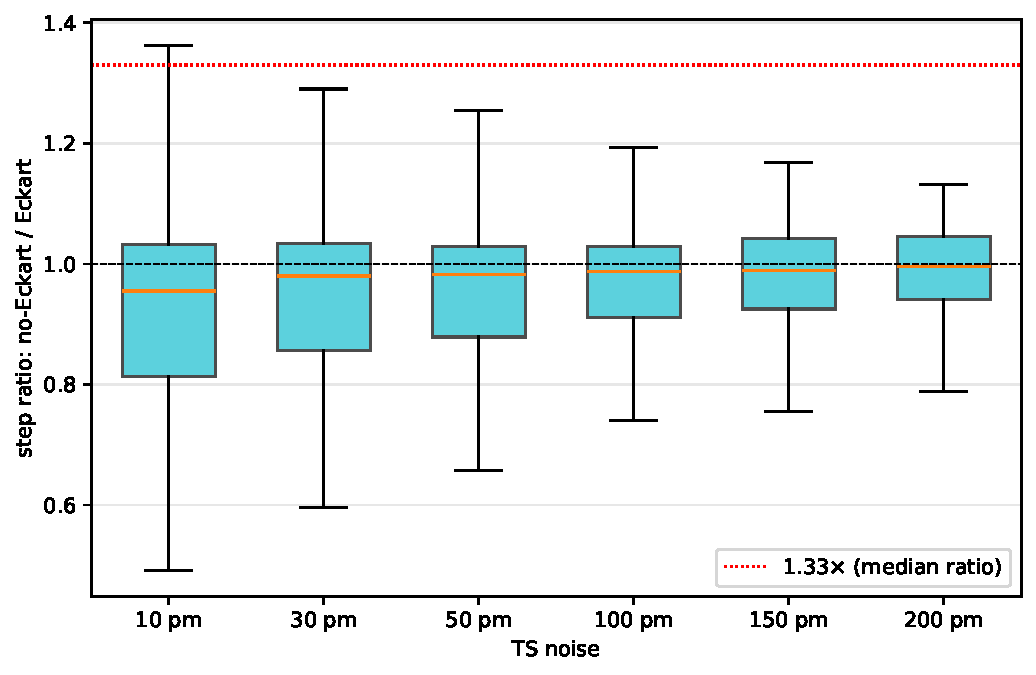
\includegraphics[width=0.85\textwidth]{figures/fig_eckart_step_ratio.pdf}
\caption{\textbf{Step ratio (no-Eckart / Eckart) per noise level, on shared
converged samples.} Boxes are 25--75 percentiles, whiskers are full
range. Median (orange line) sits at 0.91--0.97 across noise levels.
The dashed line at 1.0 is "tied"; values below indicate no-Eckart is
faster.}
\end{figure}

\subsubsection*{D. Step distributions per noise (full picture)}

\begin{figure}[H]
\centering
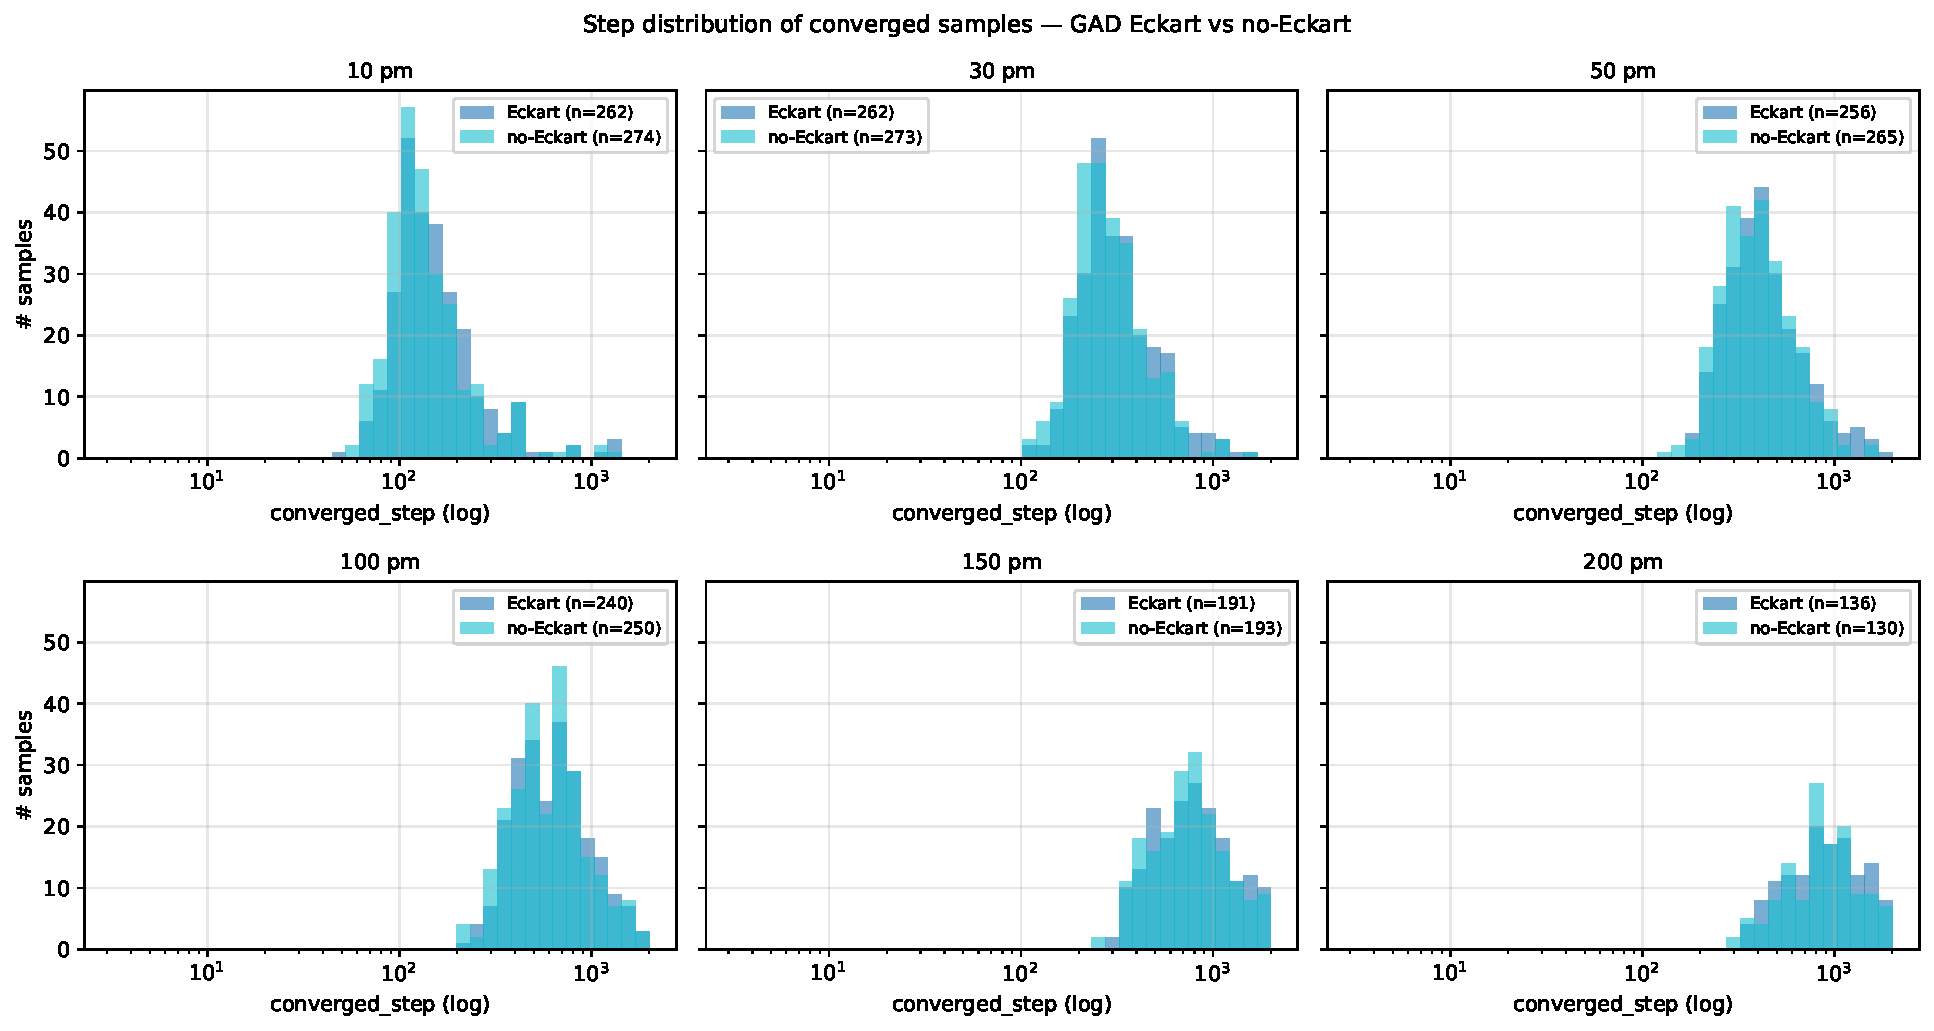
\includegraphics[width=\textwidth]{figures/fig_eckart_step_distributions.pdf}
\caption{\textbf{Distribution of \texttt{converged\_step} for samples that
converged under each method, log $x$-axis.} Eckart and no-Eckart
distributions overlap heavily; no-Eckart sits slightly to the left
(fewer steps) at every noise. The right tail at 150/200\,pm is what
drives the small differences in convergence rate.}
\end{figure}

\subsubsection*{E. Per-sample agreement, visualized}

\begin{figure}[H]
\centering
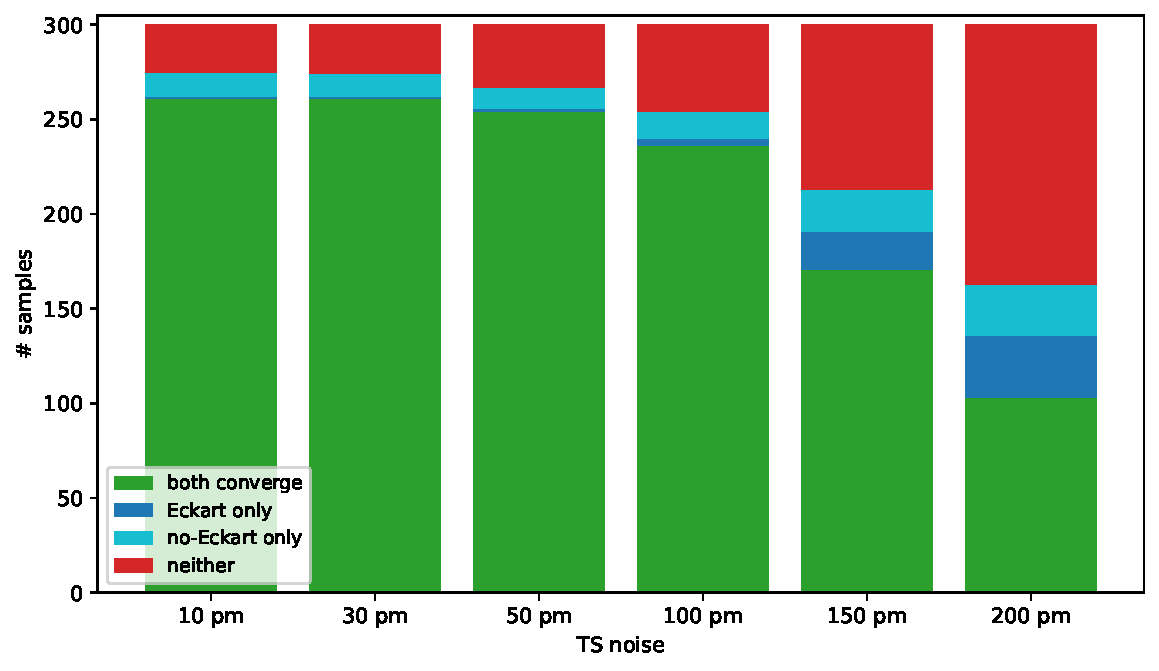
\includegraphics[width=0.85\textwidth]{figures/fig_eckart_per_sample_agreement.pdf}
\caption{\textbf{Per-noise breakdown of the 4-quadrant agreement.}
Green = converges under both; blue = only Eckart; cyan = only no-Eckart;
red = neither. Stacks always sum to 300. The cyan layer is consistently
larger than blue at low noise (no-Eckart converges more samples); the
green floor erodes from 300 down to 103 as noise grows.}
\end{figure}

\subsubsection*{F. Final TS quality is the same under both methods}

For the 261--103 samples at each noise level where both methods converge,
the median absolute lowest eigenvalue $|\lambda_0|$ at the converged TS
is essentially identical (always within 0.5 eV/\AA$^2$). Both methods
land at the same set of saddles geometrically.

\begin{center}
\begin{tabular}{rrrr}
\toprule
Noise & $|\lambda_0|$ Eckart & $|\lambda_0|$ no-Eckart & $\Delta$ \\
\midrule
10\,pm  & 4.57 & 4.50 & 0.07 \\
30\,pm  & 4.34 & 4.36 & 0.02 \\
50\,pm  & 4.12 & 4.13 & 0.02 \\
100\,pm & 4.71 & 4.73 & 0.02 \\
150\,pm & 7.45 & 7.44 & 0.01 \\
200\,pm & 8.53 & 8.30 & 0.22 \\
\bottomrule
\end{tabular}
\end{center}

\subsubsection*{G. IRC outcomes also agree}

\begin{center}
\begin{tabular}{rrrrrr}
\toprule
Noise & BOTH IRC int & E-IRC only & N-IRC only & NEITHER & agreement \\
\midrule
10\,pm  & 278 & 1  & 0  & 21  & 99.7\% \\
30\,pm  & 279 & 0  & 0  & 21  & 100.0\% \\
50\,pm  & 271 & 1  & 0  & 28  & 99.7\% \\
100\,pm & 250 & 10 & 4  & 36  & 95.3\% \\
150\,pm & 190 & 20 & 10 & 80  & 90.0\% \\
200\,pm & 114 & 27 & 23 & 136 & 83.3\% \\
\bottomrule
\end{tabular}
\end{center}

\textbf{Per-sample IRC outcomes match $>$95\% of the time at 100\,pm and
below.} The methods land at the same saddles \emph{and} those saddles
IRC to the same labeled (R, P) pair. At 150--200\,pm, divergence
appears in both directions (some samples Eckart-correct + no-Eckart-wrong,
others vice versa) suggesting that the high-noise saddles are sometimes
actually \emph{different} (different physical TSs found by the two
methods, both valid, but matching different reactions or wrong reactions).

\subsubsection*{H. The Round~1 result, re-explained}

The Round~1 ``Eckart is the main unlock'' claim came from comparing
\texttt{pure\_gad} (no-Eckart, dt=0.005, n\_steps=300) with
\texttt{gad\_projected} (Eckart, dt=0.005, n\_steps=300). The
no-Eckart numbers were near-zero at high noise. We thought Eckart was
fixing a fundamental dynamics problem.

The corrected explanation: \textbf{300 steps is too small a budget for
\emph{either} variant on hard noise levels.} If we truncate the new
\texttt{gad\_dt003\_no\_eckart} (which reaches 91.3\% at 10\,pm and
43.3\% at 200\,pm under 2000 steps) at 300 steps, we recover Round~1's
near-zero high-noise rates: 84.3/52.7/25.7/4.3/0.7/0.7\% at 10/30/50/100/150/200\,pm
(reproduced here from \S\ref{sec:eckart_brief}). And if we similarly
cap Eckart at 300 steps, we'd find rates somewhere between those
numbers and the headline 87.3/87.3/85.3/80.0/63.7/45.3 --- the
$\sim$3\,pp Eckart $\Delta$ at 2000 steps becomes much more dramatic
under tight budget purely because both distributions skew right and
many samples cluster near the cutoff.

So Round~1 was measuring \emph{step budget vs noise interaction}, not
``Eckart vs no-Eckart''. The Eckart effect under fair comparison is
small ($\pm$3\,pp) and not even consistently in Eckart's favor.

\subsubsection*{I. Mechanistic interpretation}

The textbook claim is that Eckart projection removes the 6 TR null-space
modes from the Hessian, so the lowest-eigenvalue eigenvector cannot
"leak" into TR space. The empirical data partly contradicts this:

\begin{itemize}[nosep,leftmargin=1.5em]
\item \textbf{If TR-mode contamination were a real failure mode, no-Eckart
      should fail catastrophically on samples where the lowest physical
      mode is close in eigenvalue to a TR mode.} We don't see that.
      No-Eckart converges on slightly \emph{more} samples than Eckart
      at low noise.
\item \textbf{Hypothesis: HIP's analytic Hessian is already well-conditioned.}
      The TR null-space eigenvalues are very close to zero (numerically
      $|\lambda| \sim 10^{-4}$ in our checks), well separated from
      physical modes ($|\lambda| > 10^{-2}$). The lowest-eigenvalue
      eigenvector picks the physical mode unambiguously even without
      projection.
\item \textbf{When Eckart \emph{does} flip the chosen eigenvector at
      high noise:} the projector itself depends on the current geometry.
      If GAD is on a soft saddle where two eigenvalues are close and
      bracket zero, applying Eckart can change which one is "lowest".
      The choice between two valid candidates produces the divergent
      outcomes we see at 150--200\,pm: 33 samples Eckart-only converge,
      27 samples no-Eckart-only converge.
\end{itemize}

\textbf{Practical recommendation.} Use Eckart projection (it costs
nothing extra computationally and is theoretically clean), but do
\emph{not} expect it to rescue a step-budget-limited run, and do
\emph{not} expect it to outperform raw-Hessian dynamics by more than
a few pp at any noise level we've tested.

\subsubsection*{J. Open questions}

\begin{itemize}[nosep,leftmargin=1.5em]
\item Direct measurement of TR-mode leak in the lowest eigenvector
      (would close the mechanism story).
\item Whether the small differences amplify on larger molecules (T1x
      averages 9 atoms; effects may scale).
\item Whether the picture is the same for radically different
      Hessians (DFT, semi-empirical) or whether HIP's specific
      conditioning makes Eckart redundant here.
\end{itemize}

\clearpage
\subsection{$f_{\max}$ vs $\|\mathbf{F}\|_{\text{mean}}$ criterion --- brief comparison}
\label{sec:fmax_vs_fnorm}

The historical \texttt{gad\_dt003} data uses
$\|\mathbf{F}\|_{\text{mean}} = \frac{1}{N}\sum_i |\mathbf{f}_i|$ as the
force criterion. The canonical 2026-04-20 tables use $f_{\max} = \max_i |\mathbf{f}_i|$.
For an $N$-atom molecule, $f_{\max} \geq \|\mathbf{F}\|_{\text{mean}}$ by 2--4$\times$,
so fmax<0.01 is the strict criterion. Switching from force\_norm to fmax produces a
$\sim$7\,pp drop in convergence rate, consistent across all noise levels:

\begin{center}
\begin{tabular}{rrrrr}
\toprule
Noise & force\_norm \% & fmax \% & $\Delta$ (drop, pp) \\
\midrule
10\,pm  & 94.7 & 87.3 & $-7.3$ \\
30\,pm  & 94.3 & 87.3 & $-7.0$ \\
50\,pm  & 92.0 & 85.3 & $-6.7$ \\
100\,pm & 87.3 & 80.0 & $-7.3$ \\
150\,pm & 71.3 & 63.7 & $-7.7$ \\
200\,pm & 52.3 & 45.3 & $-7.0$ \\
\bottomrule
\end{tabular}
\end{center}

\begin{figure}[H]
\centering
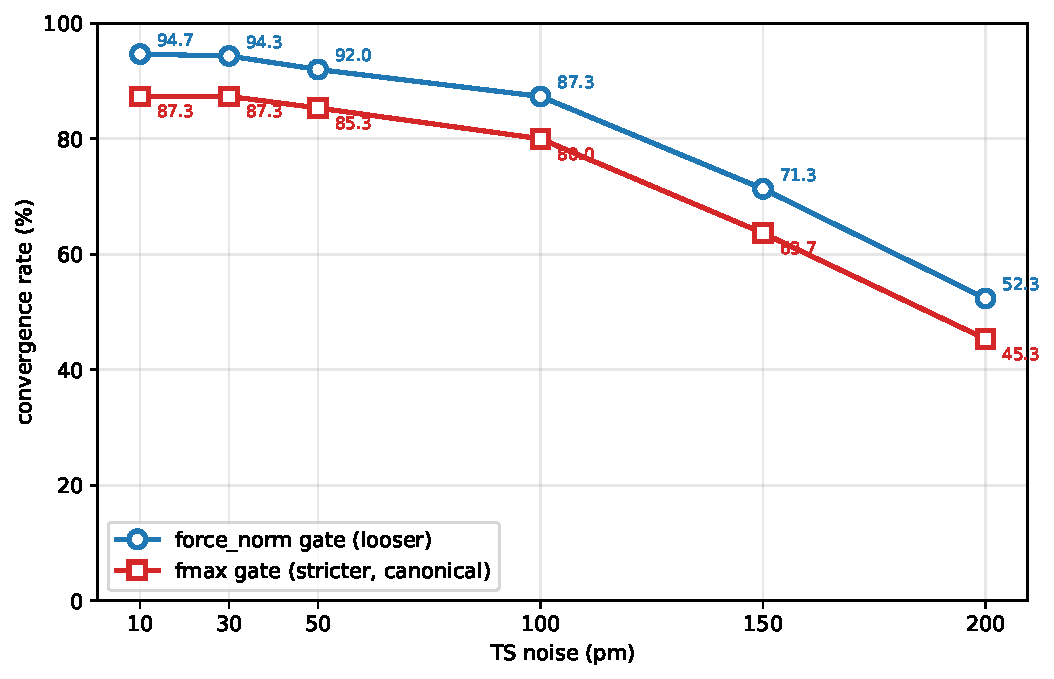
\includegraphics[width=0.7\textwidth]{figures/fig_fmax_vs_fnorm.pdf}
\caption{\textbf{GAD Eckart convergence rate under the two criteria.}
Same dynamics, same trajectories, two thresholds. The fmax criterion is the
canonical choice: it matches Sella's criterion (clean apples-to-apples)
and is more stringent (no straggling-atom force above 0.01). The
historical force\_norm row in older reports should be read as
$\sim$7\,pp upward-biased relative to a canonical fmax measurement.}
\end{figure}

\textbf{IRC outcomes are insensitive to the choice of criterion.} Validating
the same TS sets through \texttt{sella\_hip} IRC yields nearly identical
TOPO-intended rates whether we use the force\_norm-criterion set or the
fmax-criterion set: 92.7/92.7/89.7/86.3/69.7/47.9 vs 93.0/93.0/90.7/86.7/70.0/47.0.
Differences are within $\pm$1\,pp, well inside per-sample stochasticity.
This is the strongest argument that \emph{the choice of criterion does not
change the chemistry of the TS GAD finds}, only the bookkeeping of which
samples are labeled "converged".

\textbf{Recommendation.} Use $f_{\max}{<}0.01$ for all new sweeps and
all comparisons against Sella. Keep historical force\_norm data for
continuity but cite it with the explicit caveat that the rates are
$\sim$7\,pp higher than a canonical fmax measurement of the same
trajectories.

\clearpage
\subsection{Backfill: IRC on \texttt{gad\_dt002} and \texttt{gad\_projected} (2026-04-28)}

The five-method matrix in the main body omits two methods that show up in
the consolidated ranking (see \texttt{EXPERIMENT\_LOG.md} Round~7):
\texttt{gad\_dt002} (3000-step,
$dt{=}0.002$ --- the top raw TS-finder under
$\|\mathbf{F}\|_{\text{mean}}{<}0.01$) and \texttt{gad\_projected} (the
Round~1 baseline, 300-step, $dt{=}0.01$). Both pools were selected by
$\|\mathbf{F}\|_{\text{mean}}{<}0.01$, so this is also a second data
point on how much the looser criterion inflates downstream IRC.

Session: 29 array tasks dispatched, 6 retry tasks ran $\sim$16\,h
overnight at $n{=}100$ cells; 35 IRC cells produced in total.
\texttt{sella\_hip} all-endpoints, TOPO-intended.

\begin{center}
\begin{tabular}{lcccccc}
\toprule
Method & 10\,pm & 30\,pm & 50\,pm & 100\,pm & 150\,pm & 200\,pm \\
\midrule
\texttt{gad\_dt002}     & 69.0 (n=100) & 69.0 (n=100) & 61.0 (n=300) & 58.7 (n=300) & --- & --- \\
\texttt{gad\_projected} & 50.3 (n=300) & 56.0 (n=100) & 57.0 (n=100) & 55.0 (n=100) & 47.0 (n=100) & 28.3 (n=300) \\
\bottomrule
\end{tabular}
\end{center}

These rates are $\sim$20--30\,pp below the fmax-criterion GAD Eckart numbers
in the main body (92.7 / 89.7 / 86.3\,\% TOPO at 10/50/100\,pm). Both
backfill methods used the looser $\|\mathbf{F}\|_{\text{mean}}{<}0.01$
criterion, so their TS pools include marginally-converged candidates that
pass force\_norm but not fmax; those drift on IRC. This independently
confirms the recommendation in the criterion-comparison appendix:
$f_{\max}{<}0.01$ is the right criterion for downstream IRC, not just for
fair comparison with Sella. The rerun of \texttt{gad\_dt002} under fmax
is on the backburner --- expected $\sim$+25--30\,pp on IRC TOPO.

Output dirs: \texttt{runs/irc\_gad\_dt002/},
\texttt{runs/irc\_gad\_projected\_round1/}.

\clearpage
\subsection{Sella IRC halt-at-step-0 fix}

Initial Sella$\to$IRC runs on Sella-refined TSs returned trivial
results (IRC halted at step 0, wall $\approx$0.24\,s per sample). Root
cause: ASE's \texttt{Optimizer.irun} checks \texttt{gradient\_converged}
before any \texttt{step()}, and Sella's IRC halt threshold (fmax$<$0.01)
matches Sella's TS optimizer threshold exactly. So a Sella-refined TS
trivially satisfied the halt before the first kick.

Fix: \texttt{src/gadplus/search/irc\_sella\_hip.py::\_force\_first\_kick}
monkey-patches \texttt{converged}, \texttt{gradient\_converged}, and
\texttt{step} so the first convergence check always returns False.
Post-first-step behavior is unchanged.

\subsection{Data locations}

\begin{center}
\begin{tabular}{ll}
\toprule
Artifact & Path \\
\midrule
GAD dt003 (Eckart) summaries & \texttt{runs/round2}, \texttt{round3} (200\,pm refilled) \\
GAD no-Eckart summaries      & \texttt{runs/gad\_no\_eckart/} \\
Sella 2000-step (3 configs)  & \texttt{runs/sella\_2000/} \\
IRC on GAD Eckart            & \texttt{runs/irc\_sellahip\_allendpoints/} \\
IRC on GAD no-Eckart         & \texttt{runs/irc\_gad\_no\_eckart/} \\
IRC on Sella cart+Eck 2000   & \texttt{runs/irc\_sella\_carte\_2000/} \\
IRC on Sella cart 2000       & \texttt{runs/irc\_sella\_cart\_2000/} \\
IRC on Sella internal 2000   & \texttt{runs/irc\_sella\_int\_2000/} \\
IRC on \texttt{gad\_dt002}   & \texttt{runs/irc\_gad\_dt002/} \\
IRC on \texttt{gad\_projected} (Round 1) & \texttt{runs/irc\_gad\_projected\_round1/} \\
Figures                      & \texttt{figures/} \\
This report                  & \texttt{IRC\_COMPREHENSIVE\_2026-04-20.tex/pdf} \\
\bottomrule
\end{tabular}
\end{center}

\subsection{Open items}

\begin{itemize}[nosep,leftmargin=1.5em]
\item Sella internal 200\,pm IRC (final cell of the 5$\times$6 matrix) still
      computing at report time.
\item Rigorous predictor-corrector IRC sits at $\sim$52\% TOPO regardless
      of noise (on GAD Eckart converged TSs). Backburner for investigation.
\item Potential backfill of GAD Eckart numbers under $f_{\max}{<}0.01$ criterion
      for strict apples-to-apples comparison (currently uses $\|\mathbf{F}\|_{\text{mean}}$).
\end{itemize}

\end{document}
